% =============================================================
% QCLand: Query-Conditioned Landmark Localisation — MSc Thesis
% UCL Department of Computer Science
%
% MODIFIED: skeleton only, per module requirements:
%   - dissertation text (excl. title/ToC/references/appendices): 30-100pp
%   - total length (text + appendices): <= 120pp
%   - 12pt, 1.5x or double spacing
%   - code repository link required (see \CodeRepoURL below)
% Structure is a first pass based on the UCL PG Project Assessment
% Form's four marking areas (Background/Aims/Organisation,
% Difficulty/Achievement, Clarity, Analysis/Testing) and this
% project's actual experimental content. TODO once the previous-
% years' thesis template is available: align chapter/section
% granularity with department convention.
%
% MASTER PAGE BUDGET (set/revised 2026-07-22 -- per-section detail
% lives in each chapter file's own header comment, this is the
% single-source-of-truth summary):
%   Ch1 Introduction              5pp
%   Ch2 Background                12pp  (raised from 10pp)
%   Ch3 Method                    15pp
%   Ch4 Experimental Setup        7pp   (cut from 8pp)
%   Ch5 Results and Discussion    30pp
%   Ch6 Conclusion                3pp   (cut from 4pp)
%   ---------------------------------
%   Chapters total                ~73pp   (target band: 60-75pp)
%   Appendix A (reproducibility)  ~5pp    (a full per-seed results
%                                          appendix was planned but
%                                          dropped, 2026-08-13: individual
%                                          seeds are retained as
%                                          experimental replicates, while
%                                          the thesis reports their
%                                          pre-specified five-seed mean
%                                          and sample SD rather than
%                                          tabulating each run separately,
%                                          \Cref{sec:setup-multiseed})
%   Front matter (title/abstract/ack/abbrevs, ToC/LoF/LoT auto-gen)  ~3.5pp
%   ---------------------------------
%   Book total estimate           ~81.5pp  (hard cap: 120pp)
% Chapters 3 and 5 are the most likely to overrun (most subsections,
% most tables) -- watch those first if the total starts creeping up.
% =============================================================

\documentclass[12pt,a4paper]{report}

% -----------------------------------------------------------
% Packages
% -----------------------------------------------------------
\usepackage{iftex}
\ifPDFTeX
  % inputenc/fontenc are pdfTeX-engine-specific; XeLaTeX/LuaLaTeX
  % handle UTF-8 and font encoding natively and do not need them.
  % Confirm which engine your Overleaf project is set to (Menu ->
  % Compiler) before compiling -- this guard makes it work either way.
  \usepackage[utf8]{inputenc}
  \usepackage[T1]{fontenc}
\fi
\usepackage{setspace}          % line spacing control
\usepackage{float}             % fixed [H] placement for selected large floats
\usepackage[a4paper,margin=2.5cm]{geometry}
\usepackage{graphicx}
\usepackage{amsmath,amssymb}
\usepackage{booktabs}          % clean tables (\toprule/\midrule/\bottomrule)
\usepackage{tabularx}          % auto-wrapping table columns (X) -- required
\usepackage{longtable}         % tables that may span more than one page
                                % for any table with long free-text cells;
                                % plain l/c/r columns do NOT wrap and force
                                % fragile hand-inserted \\ mid-cell, which
                                % has already once broken a \Cref argument
                                % split across a manual linebreak -- always
                                % prefer X columns over hand-wrapping.
\usepackage{multirow}
\usepackage{siunitx}           % consistent number/unit formatting, e.g. \qty{9.54}{\percent} (siunitx v3+; \SI is the deprecated v2 name)
\usepackage[table]{xcolor}
\usepackage{hyperref}
\usepackage{cleveref}
\usepackage{caption}
\usepackage{subcaption}
\usepackage{seqsplit}          % break long unhyphenatable \texttt identifiers (paths, config names) instead of overflowing the margin
\usepackage{listings}          % code snippets (e.g. config excerpts)
\usepackage{algorithm}
\usepackage{algpseudocode}
\usepackage{xspace}
\usepackage{microtype}         % better justification/kerning -- free page-count savings
\usepackage[
  backend=biber,
  style=numeric,
  sorting=none
]{biblatex}
\addbibresource{references.bib}

\hypersetup{
  colorlinks=true,
  linkcolor=black,
  citecolor=black,
  urlcolor=blue,
  pdftitle={QCLand: Query-Conditioned Landmark Localisation with Vision Foundation Models for Fetal Biometry},
  pdfauthor={Nan Xu},
}

% -----------------------------------------------------------
% Formatting per module requirements
% -----------------------------------------------------------
\onehalfspacing                % switch to \doublespacing if required instead
\captionsetup{font=small}      % 1.5x-spaced captions on every table/figure
                                % look oversized otherwise -- this project
                                % has many tables, worth fixing once here.
% For any individual table that still looks cramped under 1.5x spacing,
% wrap it in \begin{singlespace}...\end{singlespace} (setspace) locally
% rather than changing the global spacing.

% -----------------------------------------------------------
% Project-specific macros — keep terminology consistent everywhere
% -----------------------------------------------------------
\newcommand{\EoMT}{EoMT\xspace}
\newcommand{\BPD}{BPD\xspace}
\newcommand{\OFD}{OFD\xspace}
\newcommand{\APAD}{APAD\xspace}
\newcommand{\TAD}{TAD\xspace}
\newcommand{\FL}{FL\xspace}
\newcommand{\NME}{NME\xspace}
\newcommand{\CodeRepoURL}{https://github.com/Flora020703/eomt-landmark-detection}

% NOTE (confirmed 2026-07-22 against the actual reference thesis title
% page the student supplied -- Bilal Sidiqi, 2023): that page prints
% BOTH the author's name AND a Candidate Number, so marking is not
% strictly anonymous at the title-page level. Settled -- no longer
% under-evidenced.
\newcommand{\StudentName}{Nan Xu}
\newcommand{\CandidateNumber}{25094226}
% NOTE (corrected 2026-07-22): the title should not foreground "EoMT"
% -- the actual contribution is a systematic empirical study/adaptation
% of a segmentation architecture, not a novel lightweight architecture
% (that was the original proposal's aim, not what was delivered).
% NOTE (revised 2026-08-13): the 2026-07-22 placeholder above still
% centred "adapting a segmentation architecture" as the subject, the
% same framing this thesis's own Ch1 Motivation was rewritten away from
% (the thesis's own query-conditioned landmark-localisation framework
% should be the subject, not the prior segmentation architecture it is
% informed by). Retitled accordingly.
% NOTE (updated 2026-08-21): student confirmed this as the formal
% dissertation title. The PDF metadata above is kept in sync.
\newcommand{\ThesisTitle}{QCLand: Query-Conditioned Landmark Localisation with Vision Foundation Models for Fetal Biometry}
% Format matches the reference title page exactly ("Supervisors: X \& Y",
% no "Dr." prefix).
\newcommand{\Supervisors}{Zhehua Mao \& Sophia Bano}
\newcommand{\Programme}{MSc Machine Learning}
\newcommand{\SubmissionDate}{7 September 2026}
% NOTE (corrected 2026-07-22): removed \WordCount -- the module
% requirements this project has actually seen specify a PAGE limit
% (dissertation text 30-100pp, total incl. appendices <=120pp), not a
% word count. Do not reintroduce a word-count declaration without a
% verified source requiring one.

\begin{document}

% -----------------------------------------------------------
% Front matter
% -----------------------------------------------------------
\pagenumbering{roman}

\begin{titlepage}
\centering

\vspace*{1cm}

\includegraphics[width=5.5cm]{figures/ucl_logo.png}\par

\vspace{1.5cm}
{\Large \ThesisTitle \par}

\vspace{2cm}
{\large \StudentName\textsuperscript{1} \par}

\vspace{1cm}
{\normalsize Candidate Number: \CandidateNumber \par}

\vspace{1cm}
{\normalsize \Programme \par}

\vspace{1cm}
{\normalsize Supervisors: \Supervisors \par}

\vspace{1cm}
{\normalsize Submission date: \SubmissionDate \par}

\vfill

{\footnotesize
\textsuperscript{1}\textbf{Disclaimer:} This report is submitted as
part requirement for the \Programme\ at UCL. It is substantially the
result of my own work except where explicitly indicated in the text.
The report may be freely copied and distributed provided the
source is explicitly acknowledged.\par}

\end{titlepage}

\chapter*{Abstract}
\addcontentsline{toc}{chapter}{Abstract}

\begin{spacing}{1.4}

Accurate fetal biometry depends on the localisation of anatomical
landmarks on standard ultrasound planes, from which measurements of
fetal growth are derived. Manual landmark placement is subject to
inter-observer variability, motivating automated landmark localisation.
Existing approaches are largely based on task-specific convolutional
architectures, whereas recent self-supervised vision foundation models
offer general-purpose visual representations learned through
large-scale pretraining. Yet adapting such representations to precise
anatomical landmark predictions without sacrificing the spatial
accuracy required for fetal biometry remains underexplored.

This thesis introduces \textbf{QCLand} (Query-Conditioned Landmark
Localisation), a framework for adapting pretrained vision foundation
models to fetal landmark localisation. For each measurement-specific
model, QCLand incorporates two learned landmark query tokens into a
pretrained vision foundation model, allowing the queries to interact
with image tokens and form landmark-specific representations through
the transformer's self-attention. A new spatial decoding head,
DeconvHeadV2, then converts these query-conditioned representations
into spatial landmark heatmaps for precise localisation. The framework
is instantiated with two self-supervised backbones, DINOv2 and DINOv3,
yielding QCLand-DINOv2 and QCLand-DINOv3.

QCLand is evaluated on five fetal biometric measurements across the
UCL and Multicentre datasets using permutation-invariant normalised
mean error (PI-NME), and is compared with reproduced HRNet-W18 and
RTMPose-s baselines. QCLand-DINOv3 achieves the lowest five-seed mean
PI-NME on all five UCL measurements. Across the two datasets and five
measurements, a QCLand variant records the lowest mean error in eight
of the ten comparisons. On Multicentre, a QCLand variant records the
lowest mean PI-NME on both abdominal measurements and femur length,
while HRNet-W18 records the lowest mean on the two head measurements.
The BPD development experiments further show that introducing
DeconvHeadV2 produces the largest observed reduction in localisation
error among the evaluated architectural modifications.

These results provide evidence that vision foundation models can be
effectively adapted for precise fetal landmark localisation when
combined with landmark-query conditioning and an appropriate spatial
decoder. QCLand emerges as a competitive alternative to purpose-built
convolutional landmark-localisation architectures, supporting
query-conditioned foundation-model adaptation as a viable route to
precise anatomical landmark localisation.

\end{spacing}

\chapter*{Acknowledgements}
\addcontentsline{toc}{chapter}{Acknowledgements}

I extend my sincere gratitude to my supervisor, Zhehua Mao, and
co-supervisor, Sophia Bano, for allowing me to work on this valuable
project. Their continuous support and guidance throughout this project
have been critical. They have been readily available to address my
queries, consistently contributing to the development of ideas that
have shaped my work. I also appreciate their commitment to dedicating
time to providing constructive feedback on my drafts.

I would also like to extend thanks to my family and friends for their
continuous support. Without their encouragement and assistance, it
would have been extremely challenging to pursue this journey.


\tableofcontents
\listoffigures
\listoftables
\chapter*{Abbreviations}
\addcontentsline{toc}{chapter}{Abbreviations}

\begin{description}
  \item[APAD] Anteroposterior Abdominal Diameter
  \item[BPD] Biparietal Diameter
  \item[DINOv2/DINOv3] Self-\textsc{DI}stillation with \textsc{NO} labels, v2/v3 (Meta AI vision backbones)
  \item[DOD] Dynamic Orientation Determination (landmark-ordering mechanism)
  \item[EoMT] Encoder-only Mask Transformer
  \item[FL] Femur Length
  \item[HRNet] High-Resolution Network
  \item[NME] Normalised Mean Error
  \item[OFD] Occipito-Frontal Diameter
  \item[PI-NME] Permutation-Invariant Normalised Mean Error
  \item[TAD] Transverse Abdominal Diameter
  \item[ViT] Vision Transformer
\end{description}


\clearpage
\pagenumbering{arabic}

% -----------------------------------------------------------
% Main matter
% -----------------------------------------------------------
\chapter{Introduction}
\label{chap:introduction}


% =================================================================
% 1.1 Fetal Biometry and Clinical Motivation
% =================================================================

\section{Fetal Biometry and Clinical Motivation}
\label{sec:intro-motivation}

Fetal biometry is the routine ultrasound measurement of fetal
anatomical structures used to estimate gestational age and monitor
fetal growth throughout pregnancy \parencite{salomon2019isuog}. This
thesis considers five landmark-defined linear measurements across
three anatomical standard planes
\parencite{divece2025multicentre}: the biparietal diameter (\BPD)
and occipito-frontal diameter (\OFD) on the head plane, the
transverse abdominal diameter (\TAD) and anteroposterior abdominal
diameter (\APAD) on the abdominal plane, and femur length (\FL) on
the femur plane. Each measurement is determined by a pair of
anatomical landmarks placed by the sonographer on a standard 2D
ultrasound image. Representative examples of the five measurements
and their landmark annotations are shown in
\Cref{fig:fetal-biometry-measurements}.

\begin{figure}[!ht]
\centering
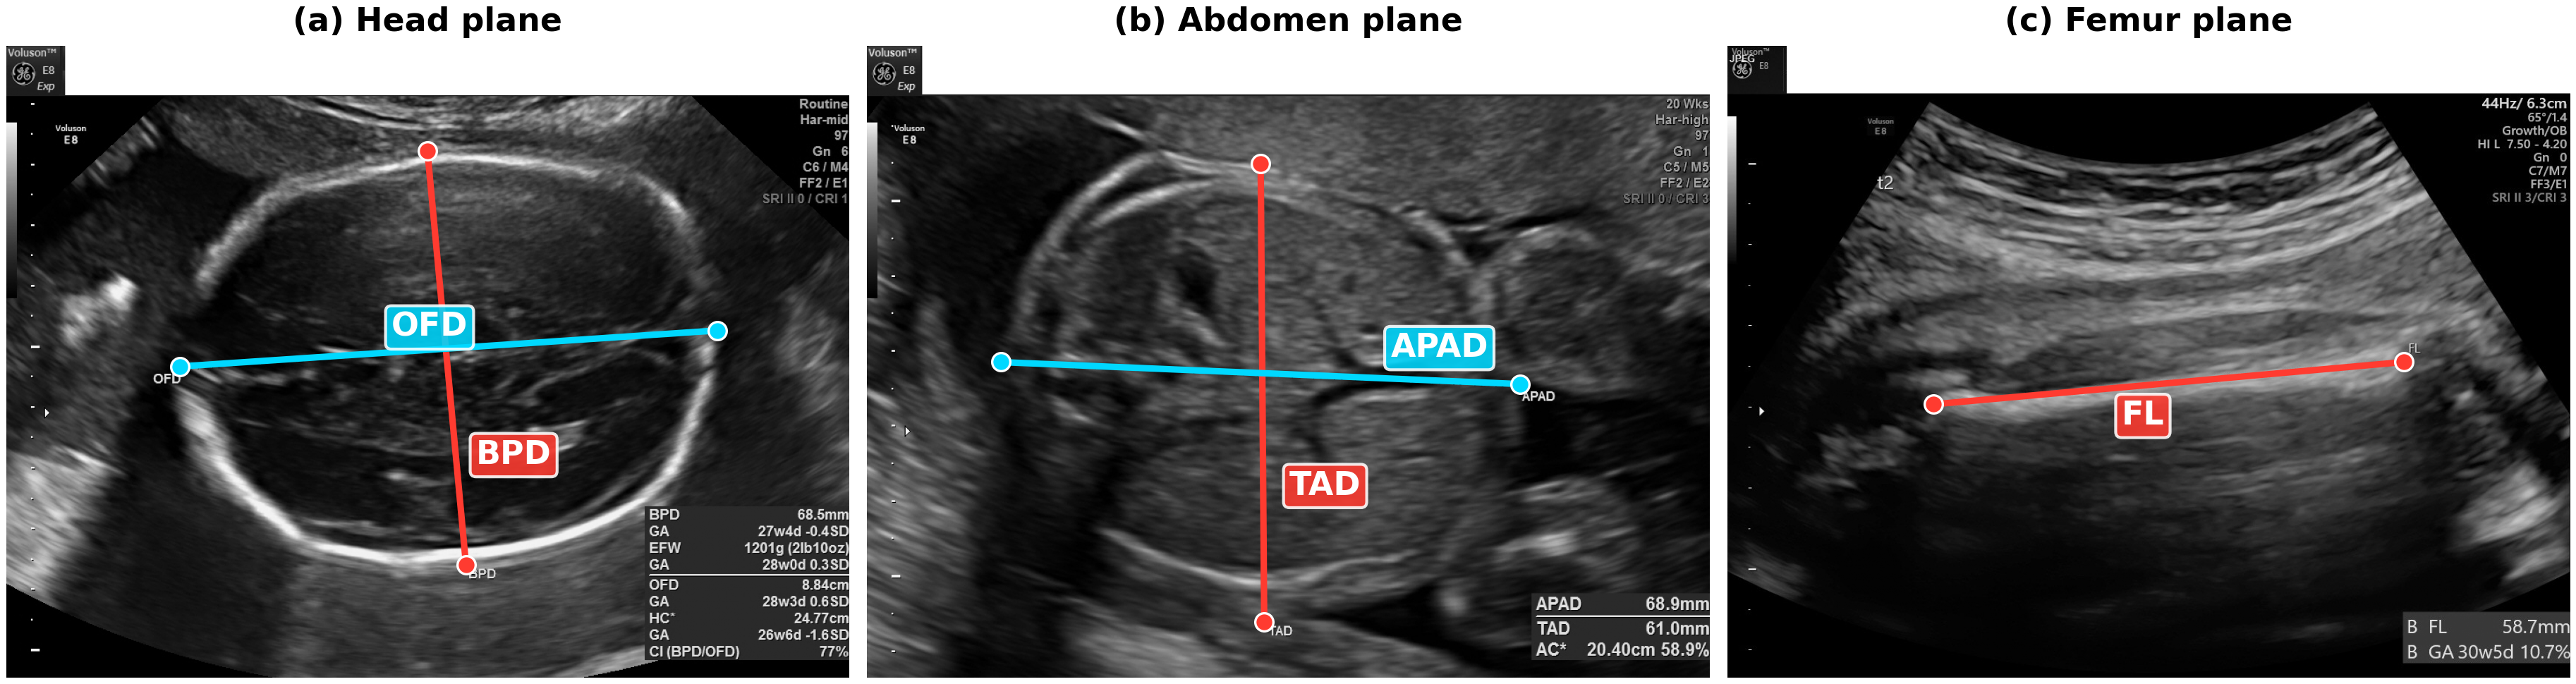
\includegraphics[width=\textwidth]
  {figures/fetal_biometry_measurements.png}
\caption{Representative fetal ultrasound images showing the five
biometric measurements considered in this thesis across the three
standard planes: (a) BPD and OFD on the head plane, (b) TAD and
APAD on the abdominal plane, and (c) FL on the femur plane. Each
measurement is defined by two anatomical landmarks, which constitute
the localisation targets in this study. Images and ground-truth
annotations are from the released UCL subset of the Multicentre
Fetal Biometry dataset \parencite{divece2025multicentre}.}
\label{fig:fetal-biometry-measurements}
\end{figure}

Manual landmark placement is not perfectly reproducible. For related
fetal measurements, \textcite{sarris2012intra} reported absolute
95\% limits of agreement ranging from 4.9\% to 11.1\% for
inter-observer differences and from 3.0\% to 6.6\% for
intra-observer differences. This operator dependence provides a
direct motivation for automated landmark localisation. Given the
same image, an automated system could reduce the variability
introduced by repeated manual landmark placement, while leaving
errors associated with image acquisition and standard-plane
selection outside its scope.


% =================================================================
% 1.2 Automated Fetal Landmark Localisation and VFMs
% =================================================================

\section{Automated Fetal Landmark Localisation and Vision Foundation
Models}
\label{sec:intro-gap}

Recent work has increasingly applied deep learning to automated fetal
biometry. P{\l}otka et al.\ developed a deep-learning approach for
automated fetal biometric measurement
\parencite{plotka2022fuvai}, while Gao et al.\ investigated
landmark-focused prediction for fetal biometry
\parencite{gao2023endpoints}. A particularly relevant formulation is
provided by the Multicentre Fetal Biometry study, which casts
biometric measurement as paired landmark localisation and provides
the principal benchmark reproduced in this thesis
\parencite{divece2025multicentre}. Its HRNet-W18-based pipeline
incorporates Dynamic Orientation Determination (DOD) to resolve the
inherent ordering ambiguity of paired landmarks.

Convolutional landmark localisation has evolved from architectures
that repeatedly aggregate multi-scale context, such as stacked
hourglass networks \parencite{newell2016hourglass}, to
deconvolutional prediction heads such as SimpleBaseline
\parencite{xiao2018simple} and high-resolution representations such
as HRNet \parencite{sun2019hrnet}. Heatmap regression has been
successfully applied to fetal biometry, while coordinate-
classification methods such as RTMPose
\parencite{jiang2023rtmpose} provide a complementary paradigm for
precise keypoint localisation. Despite their different output
formulations, these methods still rely primarily on task-specific
supervised adaptation.

Self-supervised vision foundation models shift the problem from
learning visual representations largely from task-specific
annotations to adapting representations acquired at scale. DINOv2
\parencite{oquab2023dinov2} and DINOv3
\parencite{simeoni2025dinov3} learn general-purpose visual
representations from large image corpora through self-distillation,
without requiring manual annotations for pretraining. Such
representations are attractive for fetal ultrasound, where expert
landmark annotations are costly and labelled datasets are
comparatively limited. The remaining challenge is spatial: precise
fetal biometry requires the model to form landmark-specific
representations while retaining sufficient spatial detail for
accurate localisation. How best to adapt general-purpose foundation
model representations to this setting remains underexplored.


% =================================================================
% 1.3 QCLand and Research Questions
% =================================================================

\section{QCLand and Research Questions}
\label{sec:intro-approach}

To bridge this gap, this thesis introduces \textbf{QCLand}
(Query-Conditioned Landmark Localisation), a framework that adapts
pretrained vision representations through landmark-specific query
interaction and spatial decoding. Each fetal measurement is modelled
independently: a separate QCLand model is trained for each
measurement, with two learned landmark queries corresponding to its
two landmark channels. The queries are inserted into the backbone
token sequence, allowing self-attention to form landmark-specific
representations directly through interaction with the image tokens.
This query-in-encoder formulation is inspired by recent encoder-only
query architectures \parencite{kerssies2025eomt} and is adapted here
for two-landmark localisation.

A new spatial decoding head, DeconvHeadV2, converts the
query-conditioned representations into high-resolution landmark
heatmaps for precise localisation. The framework is instantiated with
two self-supervised backbones, yielding QCLand-DINOv2 and
QCLand-DINOv3.

The thesis addresses three research questions:

\begin{description}

\item[RQ1] Can a pretrained vision foundation model be effectively
adapted for precise fetal biometry landmark localisation through
landmark-query conditioning and spatial decoding?

\item[RQ2] Which architectural adaptations are most important for
converting foundation-model representations into accurate landmark
predictions?

\item[RQ3] How does the resulting framework perform across
different fetal measurements, backbone generations
(DINOv2 vs.\ DINOv3), and the UCL and Multicentre dataset
settings, relative to established baselines?

\end{description}

The final four-model comparison provides the primary evidence for
RQ1 and RQ3 by evaluating QCLand against HRNet-W18 and RTMPose-s
across all ten dataset--measurement settings. RQ2 is investigated
through the BPD model-development study, which traces the
architectural changes leading to the adopted QCLand configuration
and examines the relative importance of the evaluated modifications.


% =================================================================
% 1.4 Contributions
% =================================================================

\section{Contributions}
\label{sec:intro-contributions}

The main contributions of this thesis are:

\begin{itemize}

\item \textbf{QCLand: query-conditioned foundation-model adaptation
for fetal landmark localisation.}
QCLand adapts pretrained DINOv2 and DINOv3 representations through
learned landmark-query interaction and spatial decoding. Its central
architectural contribution, DeconvHeadV2, replaces the inherited
dot-product readout with an explicit spatial-processing path,
providing a route from general-purpose transformer representations
to precise landmark predictions.

\item \textbf{A systematic model-development study for spatial
landmark decoding.}
Controlled experiments on BPD examine the architectural and training
changes leading to the final configuration. Among the evaluated
architectural modifications, DeconvHeadV2 produces the largest
observed reduction in localisation error, while the study also
establishes the effects and remaining uncertainties associated with
multi-depth feature fusion, pixel-centre alignment, and geometric
augmentation.

\item \textbf{Evaluation across measurements, backbones, and dataset
settings.}
QCLand-DINOv2 and QCLand-DINOv3 are evaluated across five fetal
measurements on both the UCL and Multicentre datasets against locally
reproduced HRNet-W18 and RTMPose-s baselines. The comparison uses
matched input resolution, five predefined seeds, common image
subsets, original-image-space permutation-invariant \NME{}, and
paired statistical testing. A QCLand variant achieves the lowest mean
error in eight of the ten evaluations, supporting the framework's
competitiveness across anatomical measurements and dataset settings.

\end{itemize}


% =================================================================
% 1.5 Dissertation Roadmap
% =================================================================

\section{Dissertation Roadmap}
\label{sec:intro-structure}

\Cref{chap:background} establishes the clinical and technical
context. \Cref{chap:method} defines the QCLand architecture and
training components. \Cref{chap:experimental-setup} specifies the
datasets, evaluation metric, compared models, and statistical
protocol. \Cref{chap:results} presents the comparative and ablation
results, interprets their variation across measurements and dataset
settings, and discusses the study's limitations and implications.
\Cref{chap:conclusion} summarises the findings and identifies
priorities for future work.

The implementation and reproduction scripts will be made publicly
available at
\url{https://github.com/Flora020703/eomt-landmark-detection}
upon submission.

\chapter{Background and Related Work}
\label{chap:background}

Building on the clinical motivation established in Chapter 1, this
chapter reviews the technical foundations and related work needed to
motivate QCLand. It focuses on landmark localisation paradigms,
self-supervised vision foundation models, and query-based visual
prediction.


% =================================================================
% 2.1 Fetal Biometry as a Landmark Localisation Task
% =================================================================

\section{Fetal Biometry as a Landmark Localisation Task}
\label{sec:bg-task}

For the purposes of this thesis, fetal biometry is formulated as a
two-landmark localisation problem: given a single 2D ultrasound image
of a standard plane, the task is to predict the two landmark
coordinates that define a specific measurement. This is a direct
localisation task rather than a segmentation task: the required output
is a pair of precise coordinates rather than a delineated anatomical
region or contour.

A characteristic of this formulation is landmark-ordering ambiguity.
The two landmarks defining a diameter measurement have no intrinsic
anatomical first/second identity: the same clinical measurement is
obtained regardless of which landmark is labelled first. Different
datasets may therefore adopt different ordering conventions, and a
model that correctly localises both landmarks but reports them in the
reversed order could be penalised under an order-sensitive evaluation.
This ambiguity must therefore be addressed at training time,
evaluation time, or both \parencite{divece2025multicentre}.


% =================================================================
% 2.2 Deep Learning for Landmark Localisation
% =================================================================

\section{Deep Learning for Landmark Localisation}
\label{sec:bg-landmark-methods}

Common formulations for learning-based 2D landmark localisation
include direct coordinate regression, heatmap regression, and
coordinate classification. Direct coordinate regression collapses
spatial features before predicting numeric $(x,y)$ coordinates;
DeepPose is an early deep-learning example of this formulation
\parencite{toshev2014deeppose}. Although conceptually simple, direct
regression provides less explicit spatial supervision than methods
that retain a structured spatial output, motivating the widespread
use of heatmap- and classification-based formulations.


\subsection{Heatmap Regression}
\label{sec:bg-heatmap}

In heatmap regression, a model produces a dense spatial response map
for each landmark, typically trained to approximate a Gaussian centred
on the ground-truth location
\parencite{tompson2014joint}. A coordinate can then be recovered from
the response map through a discrete maximum with optional local
refinement, or through a differentiable spatial expectation
\parencite{sun2018integral}. The key advantage of this formulation is
that it preserves an explicit correspondence between output locations
and image regions.

Heatmap regression has been developed through progressively refined
convolutional architectures. Stacked hourglass networks
\parencite{newell2016hourglass} introduced repeated
downsampling--upsampling stages with skip connections to combine local
and contextual information. SimpleBaseline
\parencite{xiao2018simple} later showed that a comparatively simple
deconvolutional head on top of a ResNet backbone
\parencite{he2016resnet} can achieve strong keypoint-localisation
performance. HRNet \parencite{sun2019hrnet} took a different approach
by maintaining high-resolution representations throughout the network.
Parallel convolutional streams at multiple resolutions repeatedly
exchange information, allowing the final landmark heatmaps to be
predicted from a high-resolution representation rather than
reconstructed only after a low-resolution bottleneck.

Beyond general pose estimation, heatmap-based localisation has also
been adopted in medical imaging, where explicit spatial modelling can
improve landmark localisation when annotated data are limited
\parencite{payer2019spatial}.


\subsection{HRNet and Landmark Ordering for Fetal Biometry}
\label{sec:bg-hrnet}

The HRNet-W18-based fetal biometry pipeline reported in the
Multicentre Fetal Biometry study
\parencite{divece2025multicentre} adapts high-resolution heatmap
regression to paired fetal landmarks. In addition to the underlying
HRNet architecture, the method incorporates Dynamic Orientation
Determination (DOD) to address landmark-ordering ambiguity. DOD
estimates a measurement-specific direction from the training data and
uses it to impose a consistent ordering on the two landmarks, reducing
errors caused solely by inconsistent annotation conventions.

Related fetal-biometry work has explored direct landmark prediction
using geometric and attention-based constraints
\parencite{gao2023endpoints}.

Together, these studies show how purpose-built landmark architectures
can accommodate the geometric structure of fetal biometry. Their
representations, however, are still learned primarily through
task-specific supervised adaptation, providing a useful contrast to
the large-scale self-supervised representations considered later in
this chapter.


\subsection{Coordinate Classification}
\label{sec:bg-simcc}

Coordinate classification avoids constructing a full two-dimensional
heatmap by discretising the horizontal and vertical axes into
classification bins and predicting a probability distribution over
each coordinate axis. SimCC \parencite{li2022simcc} formulates
keypoint localisation as two independent one-dimensional
classification problems, reducing the quadratic spatial cost of a
full 2D heatmap while permitting fine per-axis discretisation.

RTMPose \parencite{jiang2023rtmpose} builds on this formulation by
combining a CSPNeXt backbone with an RTMCC head based on SimCC
coordinate representations. RTMPose therefore provides a useful
counterpoint to heatmap regression: precise keypoint localisation can
be achieved without maintaining a dense two-dimensional output map.


\subsection{Task-Specific Supervision and Representation Learning}

The distinction between heatmap regression and coordinate
classification lies primarily in their output representations; both
still learn the downstream task through supervised adaptation, even
when initialised from ImageNet-pretrained weights. Their feature
representations are therefore shaped primarily by the labelled
downstream task.

Self-supervised vision foundation models offer a different starting
point. Rather than learning visual representations predominantly from
the downstream annotations, they first acquire general-purpose
representations through large-scale pretraining and are subsequently
adapted to the target task. This shift motivates the central question
for QCLand: whether such representations can be adapted without
sacrificing the spatial precision required for landmark localisation.


% =================================================================
% 2.3 Vision Foundation Models and Query-Based Prediction
% =================================================================

\section{Vision Foundation Models and Query-Based Prediction}
\label{sec:bg-vfm-query}

Two developments are particularly relevant to QCLand:
self-supervised vision transformers, which provide transferable
patch-level visual representations, and query-based prediction
mechanisms, which provide a way to form output-specific
representations through interaction with image features.


\subsection{Vision Transformers}
\label{sec:bg-vit}

A Vision Transformer (ViT, \textcite{dosovitskiy2021vit}) represents
an image as a sequence of fixed-size patches. Each patch is projected
into a token embedding and processed by a stack of transformer encoder
blocks using self-attention. Unlike conventional convolutional
hierarchies, a plain ViT generally maintains a single patch-token
resolution through its encoder, while self-attention allows
information to be exchanged globally across spatial locations.

This property is useful for landmark localisation because each patch
token retains an association with a spatial region while also
incorporating global image context. Features from different
transformer depths therefore share the same spatial grid while
encoding different stages of visual processing, a property that
downstream architectures can exploit.


\subsection{DINOv2 and DINOv3}
\label{sec:bg-dino}

DINOv2 \parencite{oquab2023dinov2} is a self-supervised vision
transformer trained using a teacher--student framework in which the
student is encouraged to produce representations consistent with a
momentum-updated teacher across different augmented views. The
pretraining objective does not require manual semantic annotations.
Earlier work on DINO showed that self-distilled ViTs develop both
strong recognition features and emergent spatial structure
\parencite{caron2021dino}. DINOv2 scales this approach to large,
curated image collections, producing general-purpose visual
representations that transfer effectively to downstream tasks such as
classification, segmentation, and depth estimation.

Of particular relevance to landmark localisation are DINOv2's dense
patch-level representations. Individual patch tokens remain spatially
associated with image regions while encoding increasingly contextual
visual information through the transformer layers. Such
representations provide a richer pretrained starting point for
spatial prediction than learning all visual features solely from a
small task-specific labelled dataset.

DINOv3 \parencite{simeoni2025dinov3} further scales the DINO family
and introduces changes intended to preserve the quality of dense
representations during large-scale training. Gram anchoring
regularises patch-level feature relationships during training, while
rotary position embeddings replace the learned absolute position
embeddings used by DINOv2. DINOv2 and DINOv3 therefore represent two
successive generations of self-supervised vision foundation models
that provide strong dense visual representations for downstream
adaptation.


\subsection{Query-Based Prediction: From DETR to EoMT}
\label{sec:bg-eomt}

Learned query representations have become an established mechanism for
structured visual prediction. DETR \parencite{carion2020detr}
introduced learned object queries that interact with image features
through a transformer decoder, with bipartite Hungarian matching used
to associate predictions with ground-truth objects. Mask2Former
\parencite{cheng2022mask2former} extended the query-based formulation
to segmentation, where each query predicts both a semantic category
and a spatial mask.

The Encoder-only Mask Transformer (EoMT,
\textcite{kerssies2025eomt}) simplifies this architecture by removing
the separate transformer decoder. Instead, learned mask-query tokens
are inserted directly into the ViT patch-token sequence partway
through the encoder. Subsequent transformer blocks allow queries and
image tokens to interact through the backbone's own self-attention,
so the ViT itself performs the query--image information exchange.

For spatial prediction, each EoMT query is transformed and compared
with transformed dense patch features through a per-location dot
product,

\begin{equation}
    \label{eq:bg-einsum}
    M_q(x,y)
    =
    f(q)^\top g\bigl(z(x,y)\bigr),
\end{equation}

where $q$ denotes a query representation, $z(x,y)$ is the visual
feature at spatial position $(x,y)$, and $f$ and $g$ are learned
transformations. This formulation is well matched to region-mask
prediction, but segmentation performance alone does not establish
its suitability for sharply localised landmark targets.

EoMT also applies supervision at multiple transformer depths. The
predicted masks can influence subsequent query-to-image attention,
while Hungarian matching associates a variable number of
segmentation instances with the available queries. These mechanisms
reflect the setting for which EoMT was designed:
variable-cardinality region segmentation rather than fixed-count
landmark localisation.


% =================================================================
% 2.4 Summary and Research Gap
% =================================================================

\section{Summary and Research Gap}
\label{sec:bg-summary}

The literature reviewed above brings together three complementary
lines of work. Purpose-built landmark architectures such as HRNet
provide high-resolution spatial localisation and have already been
adapted to fetal biometry, but rely primarily on task-specific
supervised training. Self-supervised vision foundation models such as
DINOv2 and DINOv3 provide general-purpose, spatially grounded patch
representations learned through large-scale pretraining, but do not
themselves produce landmark coordinates. Query-based architectures
such as EoMT allow learned queries to form output-specific
representations through interaction with ViT image tokens, but were
developed for variable-cardinality segmentation rather than precise
paired-landmark prediction.

Fetal biometry combines these requirements in a different way: each
measurement is defined by a fixed pair of landmarks, their ordering
may be ambiguous, and accurate measurement depends on spatially
precise coordinate recovery. The resulting adaptation problem is
therefore to combine query-conditioned foundation-model
representations with a spatial readout suited to precise landmark
localisation. \Cref{chap:method} introduces QCLand to address this
gap.

\chapter{Methodology}
\label{chap:method}


% =================================================================
% 3.1 QCLand Overview
% =================================================================

\section{QCLand Overview}
\label{sec:method-overview}

Chapter 2 identified a gap between the transferable representations
offered by self-supervised vision foundation models, query-based
visual prediction, and the spatial precision required for fetal
biometry landmark localisation. QCLand addresses this gap by combining
landmark-query interaction, multi-depth spatial features, and
query-conditioned heatmap decoding within a pretrained vision
transformer.

The input ultrasound image is resized to $512 \times 512$ and passed
through a pretrained DINOv2 or DINOv3 backbone, which produces a
sequence of spatially grounded patch tokens. Two learned landmark
queries, one for each landmark channel, are inserted into the token
sequence partway through the backbone. During the remaining
transformer blocks, the queries interact with the patch tokens through
the backbone's own self-attention and form landmark-specific
representations. Features from multiple backbone depths are fused into
a shared spatial representation, while the final landmark-query
embeddings retain query-specific information. DeconvHeadV2 combines
these two inputs to produce a $64 \times 64$ heatmap for each
landmark, from which the corresponding coordinate is recovered.

Each fetal measurement is modelled independently: a separate QCLand
model is trained for each measurement, with two queries representing
its two landmarks.

\Cref{fig:qcland-architecture} illustrates the complete architecture.
The remainder of this chapter describes the landmark-query backbone,
the query-conditioned spatial decoder, multi-depth feature fusion,
the training objective, coordinate handling, and the training and
inference procedures.

\begin{figure}[!ht]
  \centering
  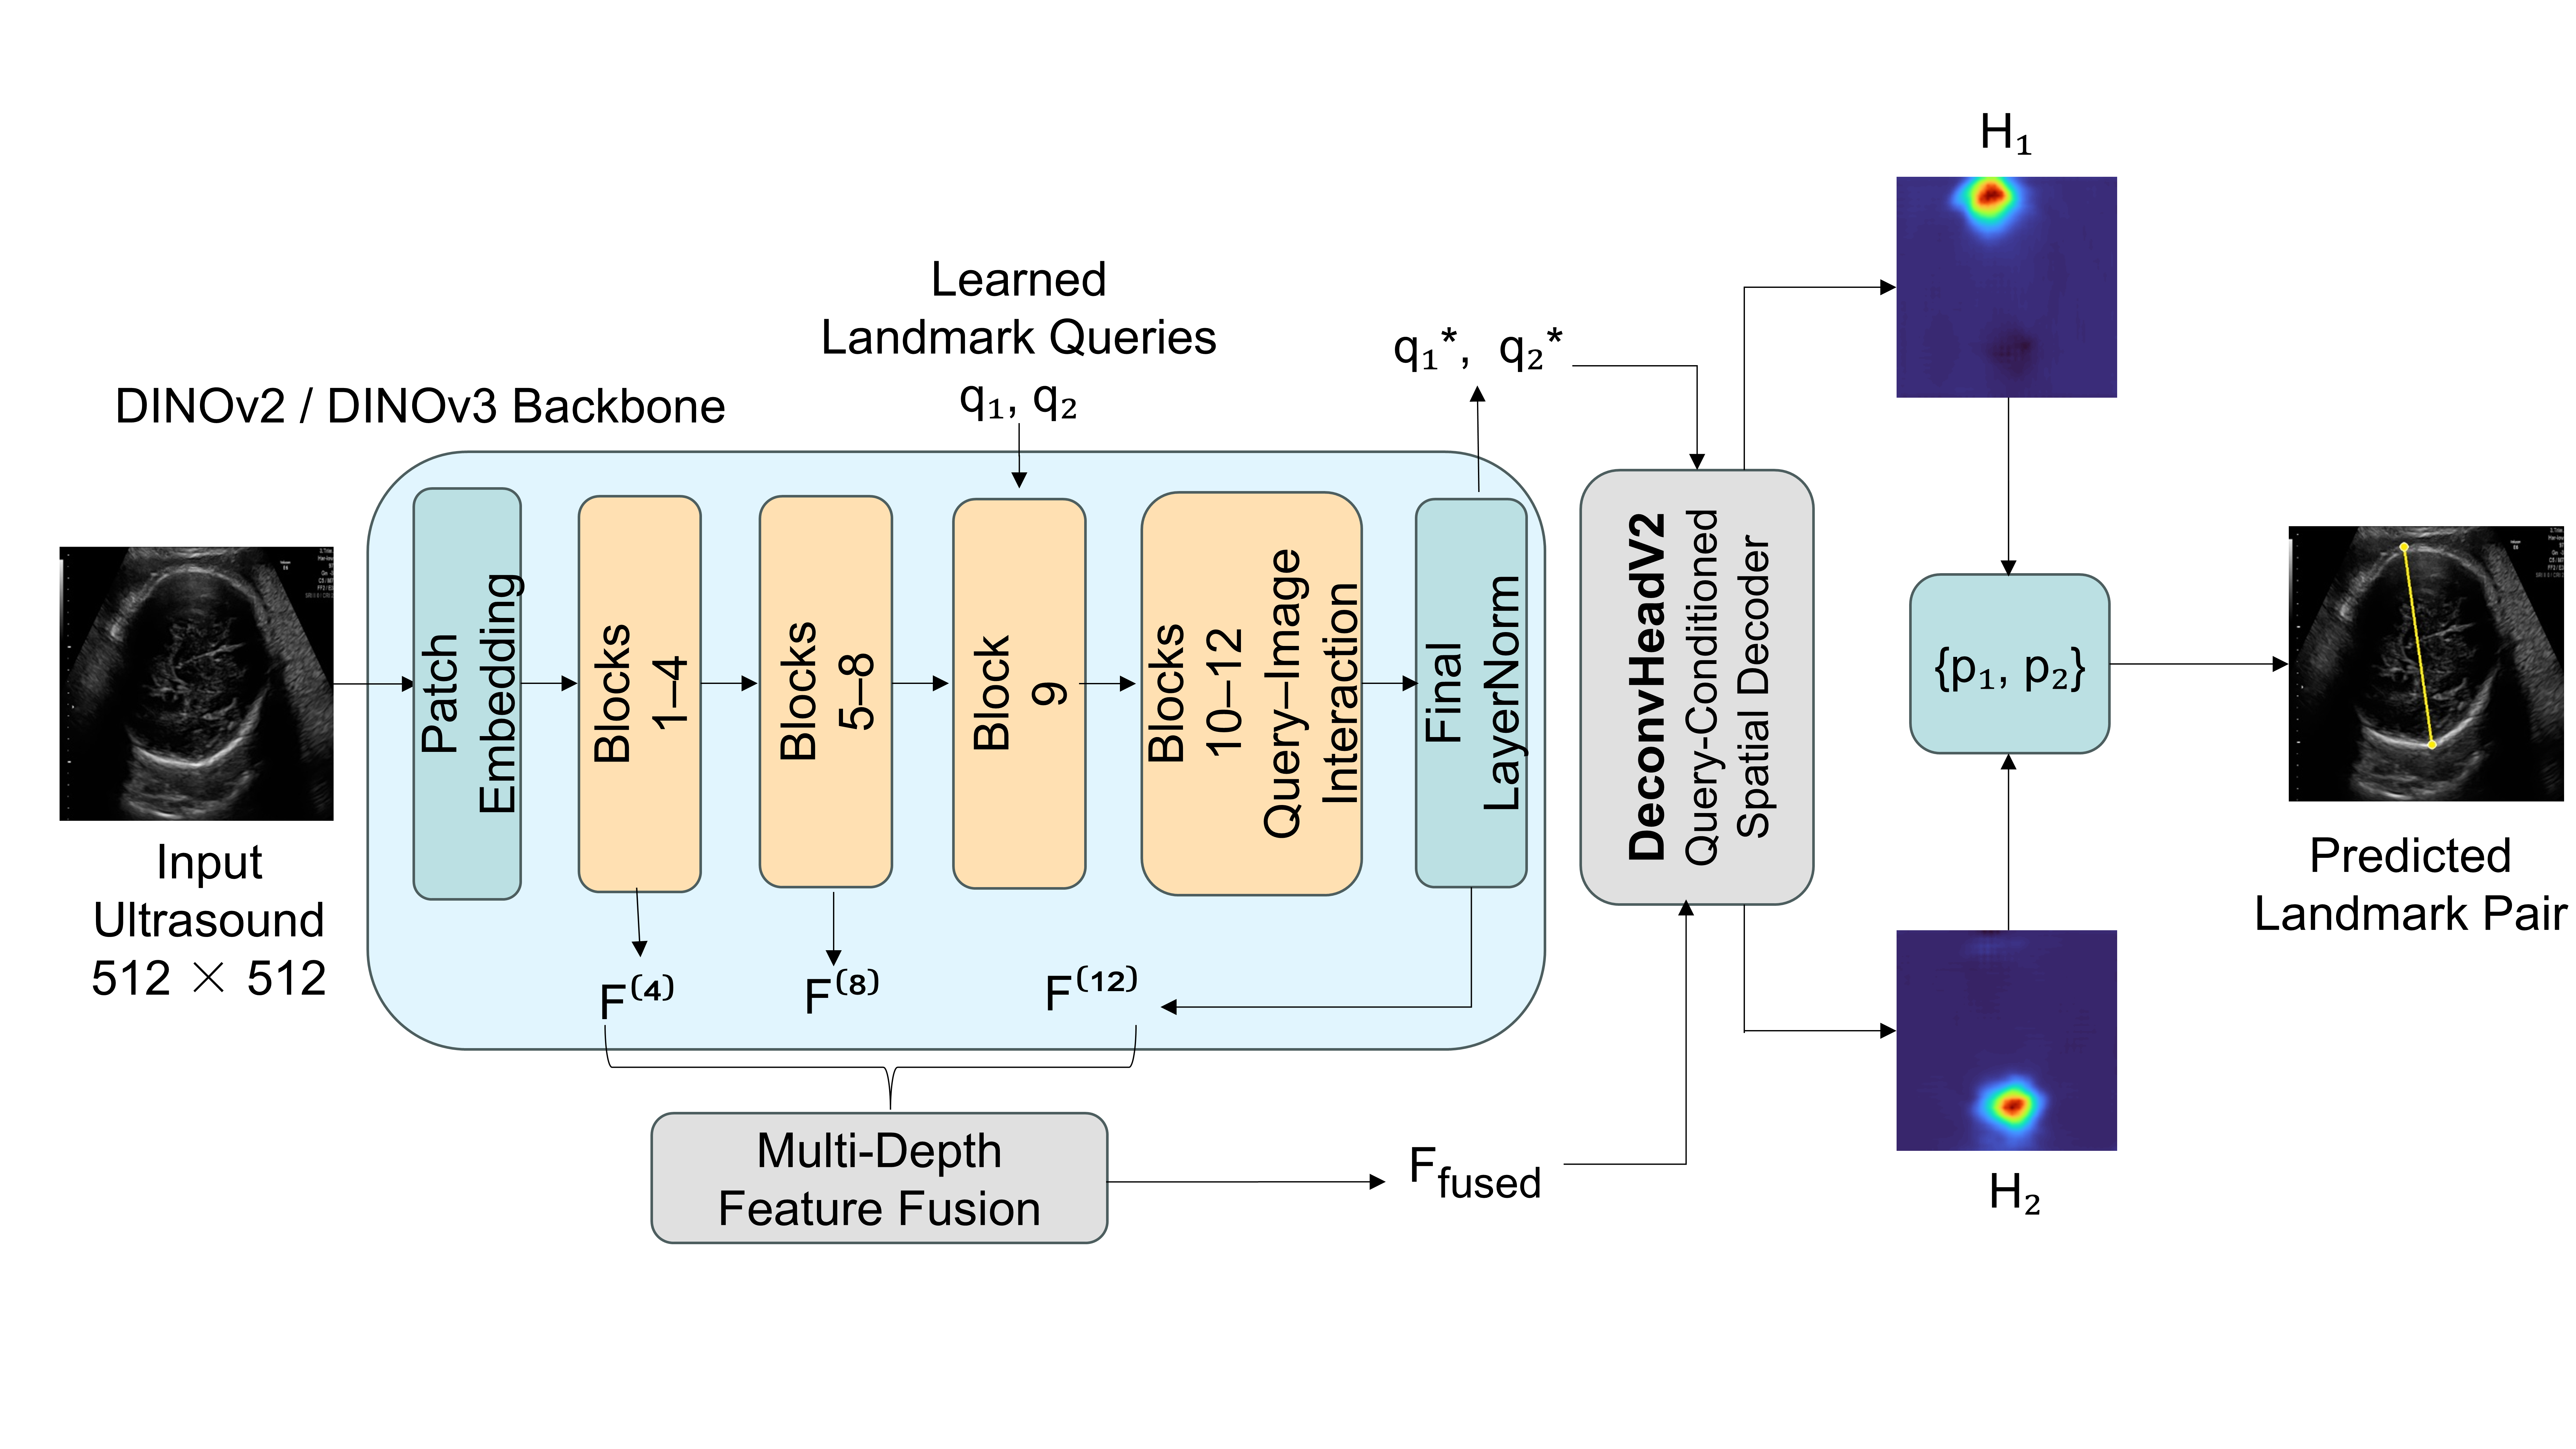
\includegraphics[width=\textwidth]
    {figures/qcland_overall_architecture.png}
  \caption[QCLand overall architecture]{Overall architecture of
    QCLand. A pretrained DINOv2 or DINOv3 backbone processes the
    input ultrasound image while two learned landmark queries
    interact with patch tokens through the final transformer blocks.
    Multi-depth patch features are fused into a shared spatial
    representation, while the final query embeddings provide
    landmark-specific conditioning. DeconvHeadV2 combines these two
    inputs to produce one heatmap for each landmark, from which the
    predicted landmark pair is recovered.}
  \label{fig:qcland-architecture}
\end{figure}


% =================================================================
% 3.2 Landmark Queries and Backbone Adaptation
% =================================================================

\section{Landmark Queries and Backbone Adaptation}
\label{sec:method-queries}

QCLand adapts a pretrained vision foundation model in two connected
ways: the backbone is fine-tuned to the fetal ultrasound domain,
while learned landmark queries are inserted into its final
transformer blocks to form landmark-specific representations. These
two components establish the representation used by the subsequent
spatial decoding stages.


\subsection{DINOv2 and DINOv3 Backbones}
\label{sec:method-backbone}

QCLand uses a pretrained vision transformer as its feature extractor.
Two backbone families are evaluated: DINOv2
\parencite{oquab2023dinov2} and DINOv3
\parencite{simeoni2025dinov3}. They share the same downstream
architecture and training framework; only the pretrained backbone
differs. The resulting variants are referred to as QCLand-DINOv2 and
QCLand-DINOv3 throughout this thesis.

Both backbones are initialised from pretrained weights and fine-tuned
jointly with the downstream QCLand components. Earlier transformer
blocks are adapted more conservatively through layer-wise
learning-rate decay, following established ViT fine-tuning practice
\parencite{bao2022beit}. For backbone block $i$ in an $L$-block
transformer,

\begin{equation}
  \label{eq:llrd}
  \mathrm{lr}_i
  =
  \mathrm{lr}_0
  \cdot
  \rho^{\,L-1-i},
\end{equation}

where $\mathrm{lr}_0 = 10^{-4}$ is the base learning rate,
$\rho = 0.8$, and $L=12$ for the backbones used here. The final block
therefore trains at the full base rate, while progressively earlier
blocks receive smaller learning rates. Non-backbone parameters,
including the landmark queries, DeconvHeadV2, and the fusion module,
are trained at the base rate. The backbone learning rate is held at
zero for the first 15 optimisation steps, allowing the newly
initialised downstream components to begin adapting before backbone
fine-tuning starts.

The DINOv2 configuration uses the ViT-S/14 register-token variant
\parencite{darcet2024registers}, with the patch-embedding kernel
resampled to $16 \times 16$ at load time. DINOv3 is natively
patch-16. Both variants therefore operate on the same
$32 \times 32$ patch-token grid for a $512 \times 512$ input,
although their positional encodings differ: DINOv2 uses learned
absolute position embeddings, whereas DINOv3 uses rotary position
embeddings.


\subsection{Landmark Queries}
\label{sec:method-landmark-queries}

Two learned query embeddings are initialised at random and inserted
into the token sequence starting $K$ blocks before the end of the
backbone, with $K=3$ in all experiments. The queries therefore
participate in blocks 10--12 together with the image and prefix
tokens. Through the backbone's own self-attention, they progressively
form landmark-specific representations by interacting directly with
the visual features.

No separate cross-attention or transformer decoder is required for
this interaction; the pretrained transformer blocks serve both as the
feature extractor and as the query--image interaction mechanism. This
query-in-encoder principle follows EoMT
\parencite{kerssies2025eomt}, while QCLand uses a fixed pair of
queries for landmark localisation.

At each of the $K$ query-interacting blocks, an auxiliary prediction
is produced using a lightweight dot-product readout
(\Cref{eq:bg-einsum}). The auxiliary predictions provide
deep-supervision loss terms during training and generate binary
attention masks that restrict each query's attention to currently
relevant image regions in the following block. Only the final
prediction, decoded through DeconvHeadV2 after the last transformer
block, is used to recover the reported landmark coordinates.


% =================================================================
% 3.3 Query-Conditioned Spatial Decoding
% =================================================================

\section{Query-Conditioned Spatial Decoding}
\label{sec:method-decoder}


\subsection{Why Spatial Decoding Is Needed}
\label{sec:method-decoder-motivation}

After the final transformer block, each landmark query contains a
representation relevant to its target landmark. Converting this
representation into a precise coordinate requires a spatial readout.
The auxiliary dot-product readout (\Cref{eq:bg-einsum}) forms each
output value independently at each spatial location, with no
subsequent local spatial mixing. Its ability to produce sharply
concentrated landmark responses is therefore not guaranteed by the
representation alone, motivating an explicit spatial decoding path
for the final prediction.


\subsection{DeconvHeadV2}
\label{sec:method-deconvheadv2}

DeconvHeadV2 is QCLand's principal architectural contribution. It
replaces the dot-product readout used for the auxiliary predictions
with a query-conditioned spatial decoding path for the final
prediction.

Before entering DeconvHeadV2, the fused spatial representation is
passed through a shared learned upsampling stage comprising two
ScaleBlocks. Each ScaleBlock doubles the spatial resolution using a
transposed convolution followed by local feature processing. Starting
from the $32 \times 32$ patch grid, the two blocks produce an
upsampled spatial representation

\[
F \in \mathbb{R}^{B \times 384 \times 128 \times 128}.
\]

DeconvHeadV2 receives this spatial representation together with the
final landmark-query embeddings. The spatial features are first
normalised using GroupNorm \parencite{wu2018groupnorm}. Each
landmark-query embedding is passed through a small MLP to predict
Feature-wise Linear Modulation (FiLM) parameters
\parencite{perez2018film}: a scale $\gamma_n$ and a shift $\beta_n$.
The normalised spatial feature map is then modulated independently for
each query:

\begin{equation}
  \label{eq:film-modulation}
  F'_n(x,y)
  =
  \gamma_n
  \odot
  \mathrm{GN}(F)(x,y)
  +
  \beta_n .
\end{equation}

The same spatial representation $F$ is therefore reused for both
landmark queries, while the query-specific FiLM parameters determine
how that representation is modulated for each landmark.

Each modulated feature map is subsequently passed through the same
shared convolutional decoder:

\begin{equation*}
  F'_n
  \xrightarrow{\;
    \mathrm{Conv}_{3\times3}
    \to
    \mathrm{ReLU}
    \to
    \mathrm{Conv}_{3\times3}
  \;}
  \widetilde{H}_n .
\end{equation*}

The first convolution reduces the channel dimension from 384 to 128,
and the second maps the 128-channel representation to a single
response map. The two landmark-query branches share these convolutional
weights; their outputs differ through the query-specific FiLM
modulation. The resulting $128 \times 128$ response map is finally
resized bilinearly to the target $64 \times 64$ landmark heatmap
$H_n$.

\Cref{fig:deconvheadv2-architecture} summarises this decoding pathway.

\begin{figure}[!ht]
  \centering
  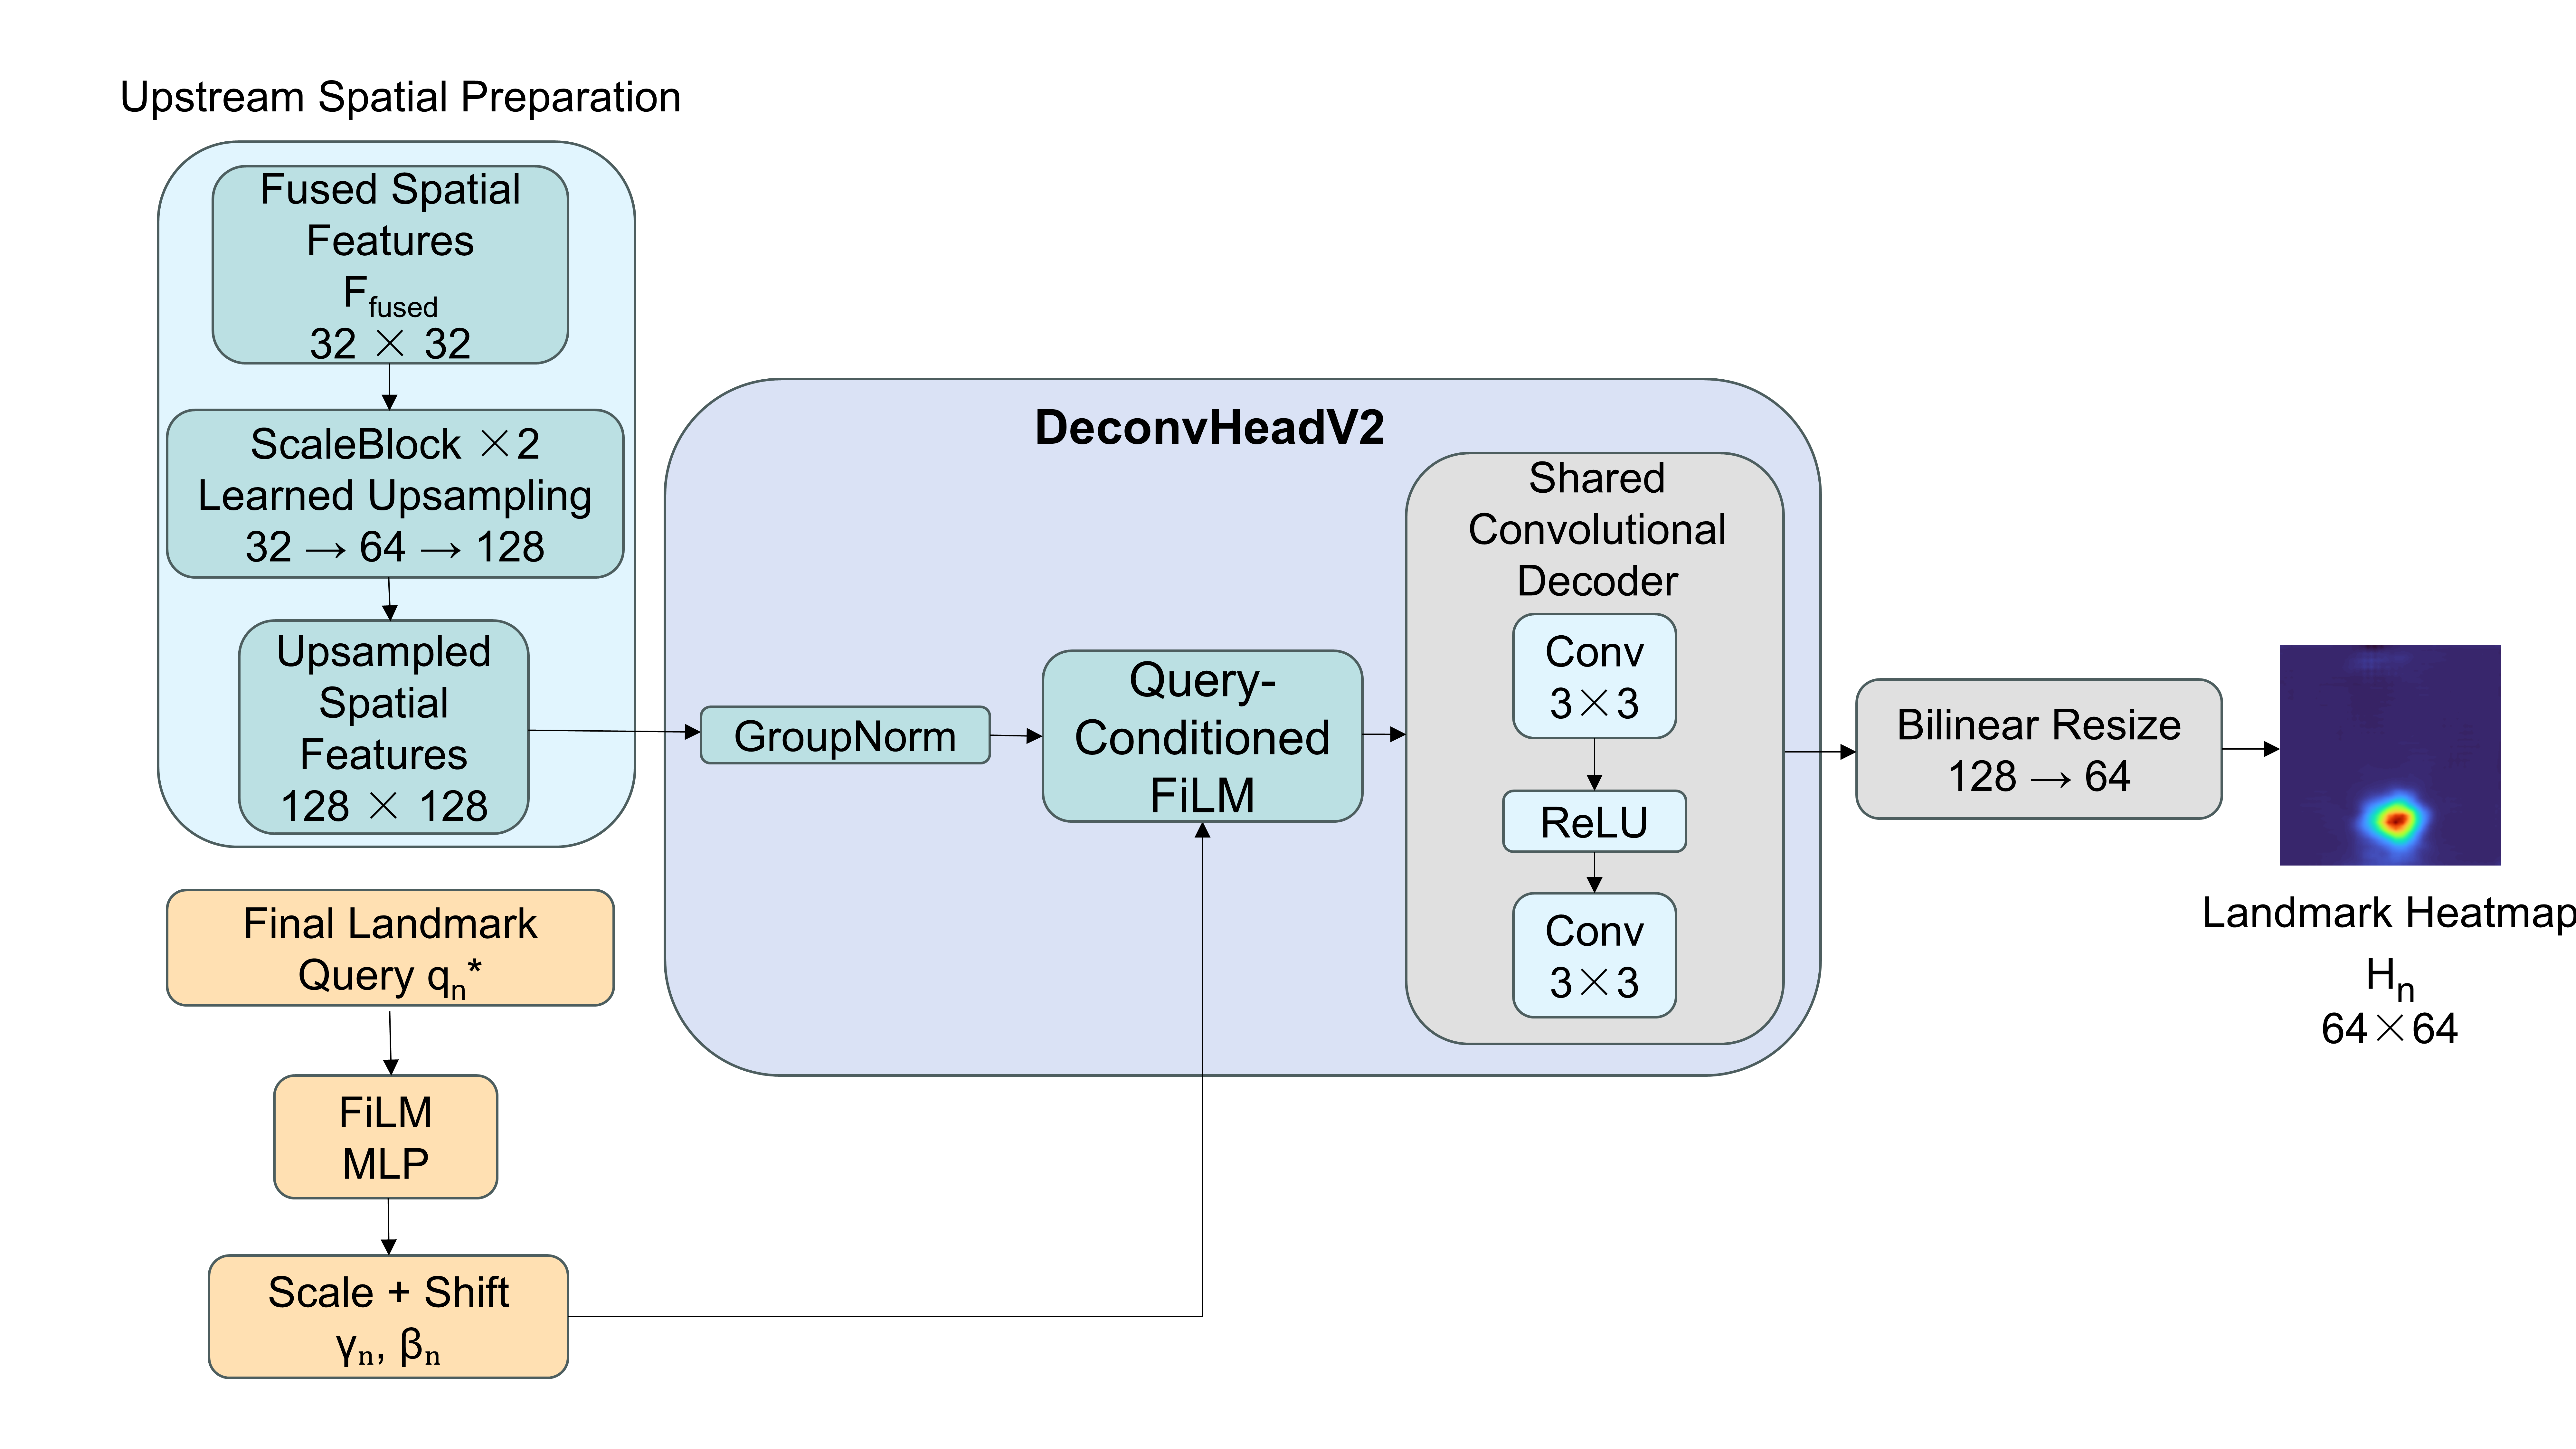
\includegraphics[width=\textwidth]
    {figures/deconvheadv2_decoding_pathway.png}
  \caption[DeconvHeadV2 decoding pathway]{DeconvHeadV2 decoding
    pathway. Fused multi-depth spatial features are first upsampled
    from $32\times32$ to $128\times128$. Inside DeconvHeadV2, the
    spatial representation is normalised and modulated by
    query-specific FiLM scale and shift parameters derived from each
    final landmark query. A convolutional decoder shared across
    landmark queries then produces a query-conditioned response map,
    which is bilinearly resized to the $64\times64$ landmark heatmap
    $H_n$.}
  \label{fig:deconvheadv2-architecture}
\end{figure}

The distinction from the auxiliary dot-product readout lies in the
spatial processing that follows query conditioning. Whereas the
dot-product formulation produces each spatial response independently,
DeconvHeadV2 applies shared convolutions over local neighbourhoods
after FiLM modulation, allowing the query-conditioned response to be
spatially refined. FiLM conditioning, GroupNorm, the shared
convolutions, and their initialisation form a single architectural
change relative to the dot-product readout; their effects are
therefore evaluated together rather than attributed to individual
subcomponents.


% =================================================================
% 3.4 Multi-Depth Feature Fusion
% =================================================================

\section{Multi-Depth Feature Fusion}
\label{sec:method-fusion}

Because a vision transformer's patch-token grid maintains the same
spatial resolution throughout the backbone, representations from
different depths remain spatially aligned while encoding different
stages of visual processing. QCLand exploits this alignment by fusing
spatial patch-token features from blocks 4, 8, and 12.

The shallower feature maps, $F^{(4)}$ and $F^{(8)}$, are captured
before the landmark queries are inserted into the token sequence.
They therefore represent image-only patch-token features at those
depths. The deepest feature map, $F^{(12)}$, is different. After the
queries are inserted before block 10, blocks 10--12 jointly process
the landmark queries, prefix tokens, and patch tokens through
self-attention. Following block 12, the backbone's final LayerNorm is
applied to the complete token sequence, after which the query and
prefix tokens are removed and the remaining patch tokens are reshaped
into a spatial feature map. Accordingly, $F^{(12)}$ denotes the
post-LayerNorm spatial patch-token features extracted after
query--image interaction through blocks 10--12.

QCLand therefore combines two pre-query representations,
$F^{(4)}$ and $F^{(8)}$, with the deepest query-interacted
representation, $F^{(12)}$. Blocks 4, 8, and 12 provide approximately
evenly spaced depths across the 12-block backbone; their selection was
not obtained through a search over alternative depth combinations.

Each feature map is independently normalised with GroupNorm. The three
normalised representations are concatenated along the channel
dimension and projected back to the backbone embedding dimension using
a $1 \times 1$ convolution. Because all three feature maps share the
same spatial grid, no top-down resizing pathway is required, unlike
the convolutional feature-pyramid architecture that motivated the
general multi-level fusion principle \parencite{lin2017fpn}.

The $1 \times 1$ projection is initialised such that only the deepest
feature level contributes at the start of training. The shallower
representations must therefore acquire useful fusion weights during
optimisation rather than perturbing the pretrained deepest
representation immediately.


% =================================================================
% 3.5 Landmark Targets and Training Objective
% =================================================================

\section{Landmark Targets and Training Objective}
\label{sec:method-objective}


\subsection{Heatmap Targets}
\label{sec:method-targets}

Following standard heatmap-based landmark supervision
\parencite{tompson2014joint,newell2016hourglass}, each landmark's
training target is a 2D Gaussian centred on the ground-truth
location, truncated to zero outside a square window of half-width
$\lfloor 3\sigma \rfloor$ pixels:

\begin{equation}
  \label{eq:gaussian-target}
  T_n(x,y) =
  \begin{cases}
    \exp\!\left(
      -\dfrac{
        (x-\mu_{x,n})^2 + (y-\mu_{y,n})^2
      }{2\sigma^2}
    \right),
    &
    |x-\mu_{x,n}|,\,
    |y-\mu_{y,n}|
    \le
    \lfloor 3\sigma \rfloor,
    \\[4pt]
    0,
    &
    \text{otherwise},
  \end{cases}
\end{equation}

where $(\mu_{x,n},\mu_{y,n})$ is the nearest heatmap pixel to the
continuous ground-truth coordinate and $\sigma=4.0$ for all fetal
experiments. The target is unnormalised with peak value 1.


\subsection{Hybrid Heatmap--Coordinate Loss}
\label{sec:method-losses}

The training objective combines a weighted heatmap term with a
coordinate-space term. The heatmap term reweights the per-pixel
squared error according to the target response:

\begin{equation}
  \label{eq:wmse}
  L_{\text{hm}}
  =
  \frac{1}{BNHW}
  \sum_{b,n,x,y}
  \bigl(1+\alpha T_{b,n}(x,y)\bigr)
  \bigl(
    \hat{H}_{b,n}(x,y)-T_{b,n}(x,y)
  \bigr)^2 .
\end{equation}

With $\alpha=5.0$, pixels at the target peak receive six times the
weight of background pixels. This foreground--background imbalance is
a known issue in landmark heatmap regression
\parencite{wang2019awing}: most locations in a $64\times64$ target
map are close to zero, so an unweighted objective can make globally
weak responses comparatively inexpensive.

A coordinate prediction is additionally extracted using a
differentiable spatial expectation (soft-argmax)
\parencite{sun2018integral}:

\begin{equation}
  \label{eq:soft-argmax}
  \hat{p}_n^{\text{soft}}
  =
  \sum_{x,y}
  (x,y)
  \cdot
  \frac{
    \exp(\tau\hat{H}_n(x,y))
  }{
    \sum_{x',y'}
    \exp(\tau\hat{H}_n(x',y'))
  },
\end{equation}

with temperature $\tau=10$. An L1 loss between this soft-decoded
coordinate and the continuous ground-truth coordinate provides a
direct spatial-precision signal:

\begin{equation}
  \label{eq:hybrid-loss}
  L
  =
  L_{\text{hm}}
  +
  \lambda_{\text{coord}}
  \cdot
  \frac{1}{2BN}
  \sum_{b,n}
  \left\lVert
    \hat{p}_{b,n}^{\text{soft}}
    -
    p_{b,n}
  \right\rVert_1,
  \qquad
  \lambda_{\text{coord}}=0.1 .
\end{equation}

The heatmap target is centred on a quantised pixel location, whereas
the coordinate term is supervised against the original continuous
coordinate. The two terms therefore provide complementary
supervision: the heatmap term shapes the spatial response, while the
coordinate term retains localisation information that heatmap
quantisation would otherwise discard.

The overall training loss is the equal-weighted average of $K+1$
per-layer terms: $K=3$ auxiliary dot-product losses and one
DeconvHeadV2 loss, each computed using the hybrid objective above.


% =================================================================
% 3.6 Coordinate Handling and Landmark Assignment
% =================================================================

\section{Coordinate Handling and Landmark Assignment}
\label{sec:method-coordinates}


\subsection{Landmark Assignment}
\label{sec:method-formulation}

The two landmarks defining each fetal measurement are treated as an
unordered pair for evaluation and do not carry persistent
query-specific anatomical identities in the training formulation.
During training, the pair is canonicalised from left to right by
$x$-coordinate in the current image coordinate system
\emph{after} any geometric augmentation has been applied. Query 0 is
assigned to the landmark with the smaller $x$-coordinate and query 1
to the landmark with the larger $x$-coordinate. The assignment is
recomputed for every sample and therefore does not encode a persistent
anatomical identity for either query.

For measurements whose two landmarks have little horizontal
separation, small geometric perturbations can reverse this ordering,
causing the same anatomical landmark to be assigned to different
queries across augmented views of an image. This behaviour follows
from the training-time canonicalisation rather than from an ambiguity
in the clinical measurement itself. Because the ordering convention
has no independent clinical meaning, evaluation treats the predicted
and ground-truth landmarks as unordered pairs using the
permutation-invariant metric defined in \Cref{sec:setup-nme}.


\subsection{Pixel-Centre-Aligned Coordinate Mapping}
\label{sec:method-udp}

Converting a landmark coordinate between the original image, the
resized model input, and the heatmap requires rescaling by the ratio
of the corresponding resolutions. A naive proportional rescaling
introduces a systematic offset because image-resizing operations treat
each pixel as covering a continuous interval centred at $x+0.5$,
rather than as a point located exactly at $x$. Following the analysis
of this class of bias by \textcite{huang2020udp}, QCLand uses a
pixel-centre-aligned mapping:

\begin{equation}
  \label{eq:udp-scale}
  x'
  =
  (x+0.5)\cdot s - 0.5,
\end{equation}

where $s$ denotes the ratio between the target and source resolutions
along the corresponding axis. The mapping is applied when encoding
annotations from original-image space to model-input and heatmap
space, and its algebraic inverse is used when recovering predictions
in original-image coordinates. The same convention is therefore used
consistently during both target construction and evaluation.


% =================================================================
% 3.7 Training and Inference
% =================================================================

\section{Training and Inference}
\label{sec:method-training}


\subsection{Data Augmentation}
\label{sec:method-augmentation}

Two layers of data augmentation are used. The baseline augmentation
applies horizontal flipping and colour jitter in brightness, contrast,
and saturation, each independently with probability 0.5. The final
QCLand configuration additionally applies rotation drawn from
$[-30^\circ,30^\circ]$ with probability 0.6 and scale jitter of
$\pm25\%$, sampled for every training image.

If a geometric transform would move any landmark outside the image,
that sample's augmentation is skipped rather than clamping the
landmark to the image boundary. The realised augmentation
distribution therefore depends on the landmark geometry of each
sample.


\subsection{Inference and Coordinate Recovery}
\label{sec:method-inference}

At inference time, the input image passes through the complete QCLand
forward path. Each predicted heatmap is decoded into a coordinate by
taking its discrete maximum and applying the conventional
quarter-pixel local refinement used in heatmap-based pose estimation
\parencite{xiao2018simple,huang2020udp}:

\begin{equation}
  \label{eq:coord-decode}
  \hat{p}_n
  =
  \begin{pmatrix}
    x_i
    +
    0.25\,
    \mathrm{sign}
      \bigl(\partial_x\hat{H}_n\bigr)
    \cdot
    \mathbb{1}[0<x_i<w-1]
    \\[4pt]
    y_i
    +
    0.25\,
    \mathrm{sign}
      \bigl(\partial_y\hat{H}_n\bigr)
    \cdot
    \mathbb{1}[0<y_i<h-1]
  \end{pmatrix},
\end{equation}

where

\[
(x_i,y_i)
=
\arg\max_{x,y}
\hat{H}_n(x,y),
\]

and $\partial_x$ and $\partial_y$ are finite differences between
adjacent heatmap values. Refinement is applied independently along
each axis, so a peak lying on the boundary of one axis can still be
refined along the other. The decoded landmark coordinates are then
mapped from heatmap space back to the original image using the inverse
pixel-centre-aligned transformation defined above.

Together, these components define the complete QCLand pipeline from
pretrained visual representation to landmark-specific spatial
prediction. Chapter 4 establishes the datasets, baseline models,
checkpoint conventions, repeated-run protocol, and evaluation
methodology used to assess the resulting framework.

\chapter{Experimental Setup}
\label{chap:experimental-setup}

Chapter 3 defined QCLand's architecture, training objective, and
inference procedure. This chapter specifies how the framework is
evaluated. It describes the datasets and their released partitions,
defines the evaluation metric, identifies the compared models,
establishes the shared protocol for the final four-model comparison,
and separates the BPD development experiments from the cross-model
evaluation.


% =================================================================
% 4.1 Datasets and Data Splits
% =================================================================

\section{Datasets and Data Splits}
\label{sec:setup-datasets}

All experiments use publicly released, de-identified fetal ultrasound
data from the Multicentre Fetal Biometry benchmark
\parencite{divece2025multicentre}. No new patient data or annotations
were collected. The pooled release was used under its CC~BY-NC-SA~4.0
licence for non-commercial academic research; original images are not
redistributed with this thesis. Ethical approvals for the constituent
datasets are recorded in \Cref{app:ethics}.


\subsection{UCL Single-Site Dataset}
\label{sec:setup-ucl}

Experiments cover the five fetal measurements introduced in
Chapter 1, with BPD/OFD sharing the Head images, TAD/APAD sharing
the Abdomen images, and FL using the Femur images. Each measurement
is defined by two anatomical landmarks per image. The experiments
retain the official Train/Test partitions released by
\textcite{divece2025multicentre} without modification.

For early stopping and checkpoint selection, a portion of each
official training pool is held out for internal validation. The split
is made over filename-prefix groups, with all frames sharing a leading
numeric prefix assigned to the same partition, using a fixed split
seed of 42. The last
$\lceil 0.1 \times n_{\text{groups}}\rceil$ groups form the
validation set. A filename-prefix group therefore cannot occur in
both the optimisation and validation sets. The exact image counts are
reported in \Cref{tab:full-dataset-sizes}.


\subsection{Pooled Multicentre Dataset}
\label{sec:setup-multicentre}

The Multicentre release \parencite{divece2025multicentre} pools UCL
with two further sources: FP, collected at two hospitals in Barcelona,
and HC18, collected at a clinical site in the Netherlands
\parencite{vandenheuvel2018hc18}. Together, the release spans four
clinical sites and seven ultrasound device models.
\Cref{tab:multicentre-per-source} shows the per-source composition.

\begin{table}[htbp]
  \centering
  \caption{Per-source image counts (Train / Test) in the pooled
    Multicentre release, by anatomy.}
  \label{tab:multicentre-per-source}
  \begin{tabular}{lccc}
    \toprule
    Anatomy & FP & HC18 & UCL \\
    \midrule
    Head     & 757 / 880 & 737 / 262 & 110 / 49 \\
    Abdomen  & 568 / 125 & --        & 94 / 36  \\
    Femur    & 437 / 323 & --        & 96 / 39  \\
    \bottomrule
  \end{tabular}
\end{table}

Internal validation groups are sampled from each pooled training
split using a fixed seed of 42 and source-aware filename grouping.
The released Train/Test partition itself is retained unchanged.
Because the pooled benchmark concatenates source-specific partitions
rather than holding out an entire clinical site, the Multicentre
experiments assess performance within the released multi-site
benchmark rather than unseen-site transfer.

\begin{table}[htbp]
  \centering
  \caption{Exact image counts for every dataset configuration used
    in this thesis.}
  \label{tab:full-dataset-sizes}
  \begin{tabular}{lcccc}
    \toprule
    Dataset (task) & Official pool & Optimisation & Validation & Test \\
    \midrule
    UCL Head (\BPD/\OFD)     & 110  & 100  & 10  & 49 \\
    UCL Abdomen (\TAD/\APAD) & 94   & 85   & 9   & 36 \\
    UCL Femur (\FL)          & 96   & 84   & 12  & 39 \\
    Multicentre Head         & 1604 & 1453 & 151 & 1191 \\
    Multicentre Abdomen      & 662  & 590  & 72  & 161 \\
    Multicentre Femur        & 533  & 481  & 52  & 362 \\
    \bottomrule
  \end{tabular}
\end{table}


% =================================================================
% 4.2 Evaluation Metric
% =================================================================

\section{Evaluation Metric}
\label{sec:setup-nme}

The two landmarks defining each fetal measurement form an unordered
pair: exchanging their labels does not change the underlying clinical
measurement. The final comparison therefore uses
permutation-invariant normalised mean error (PI-NME), allowing all
methods to be evaluated independently of their internal landmark
ordering conventions.

For predicted landmarks $\hat{p}_0,\hat{p}_1$ and ground-truth
landmarks $p_0,p_1$, the two possible correspondences are

\begin{align}
  d_{\text{direct}}
  &=
  \lVert \hat{p}_0 - p_0 \rVert_2
  +
  \lVert \hat{p}_1 - p_1 \rVert_2,
  \\
  d_{\text{crossed}}
  &=
  \lVert \hat{p}_0 - p_1 \rVert_2
  +
  \lVert \hat{p}_1 - p_0 \rVert_2.
\end{align}

With

\begin{equation}
  D = \lVert p_0 - p_1 \rVert_2,
\end{equation}

PI-NME is defined as

\begin{equation}
  \label{eq:pi-nme}
  \mathrm{PI\text{-}NME}
  =
  \frac{
    \min(d_{\text{direct}},\,d_{\text{crossed}})
  }{2D}.
\end{equation}

All distances are computed in the original image coordinate system.
Predicted coordinates are first mapped back from model-input space
using each method's own inverse geometric transform, and only then
are the two possible correspondences and final PI-NME evaluated.
This is important because the original ultrasound frames are
generally non-square, whereas the compared models operate on square
resized inputs; computing Euclidean errors directly in resized
coordinates would distort the relative contributions of the
horizontal and vertical axes.

This external PI-NME definition is applied identically to QCLand,
HRNet-W18, and RTMPose-s in the final comparison. HRNet-W18 retains
its DOD-based landmark-ordering mechanism, while the other methods
retain their own internal assignment conventions; these internal
choices do not alter the common permutation-invariant metric used
for final evaluation.


% =================================================================
% 4.3 Compared Methods and Baselines
% =================================================================

\section{Compared Methods and Baselines}
\label{sec:setup-baselines}

The final comparison includes four models: QCLand-DINOv2,
QCLand-DINOv3, HRNet-W18, and RTMPose-s. The two QCLand variants
share the architecture defined in Chapter 3 and differ only in the
pretrained backbone.


\subsection{Locally Reproduced HRNet-W18}

HRNet-W18 is reproduced from the original authors' implementation
using the released training protocol. The upstream procedure monitors
the official test partition during training rather than constructing
a separate internal validation set, and the final-state checkpoint is
used for evaluation. This differs from QCLand and RTMPose-s, which
reserve part of the training pool for internal validation. Full
reproduction details and software compatibility modifications are
documented in \Cref{app:reproducibility}.

Published BiometryNet results from
\textcite{divece2025multicentre} are retained only as contextual
references rather than protocol-matched comparisons, because their
complete training and evaluation conditions cannot be independently
matched to the present experiments.


\subsection{RTMPose-s}
\label{sec:setup-rtmpose}

RTMPose-s \parencite{jiang2023rtmpose} is adapted as a two-landmark
model trained independently for each dataset--measurement setting,
matching QCLand's and HRNet-W18's per-measurement organisation. Its
native CSPNeXt-s backbone and RTMCC/SimCC formulation are retained;
input resolution, data partitions, seeds, and external evaluation
are aligned with the final comparison protocol.

RTMPose-s trains for a fixed 200 epochs with no early stopping.
Its internal validation measurements are diagnostic only, and the
final training state is reported. The full adaptation protocol,
including codec configuration and software versions, is documented
in \Cref{app:reproducibility}.


% =================================================================
% 4.4 Final Four-Model Comparison Protocol
% =================================================================

\section{Final Four-Model Comparison Protocol}
\label{sec:setup-final-comparison}
\label{sec:setup-four-model}

The four models are compared across all ten dataset--measurement
settings: five measurements on UCL and the same five measurements
on Multicentre. \Cref{tab:comparison-conditions} summarises the
shared and method-specific evaluation conditions.

\begin{table}[htbp]
  \centering
  \caption[Four-model comparison protocol.]
  {Harmonised and method-specific conditions for the final
    four-model comparison.}
  \label{tab:comparison-conditions}
  \small
  \begin{tabularx}{\textwidth}{
    @{}>{\raggedright\arraybackslash}p{0.22\textwidth}
    *{4}{>{\centering\arraybackslash}X}@{}}
    \toprule
    Condition &
    QCLand-v2 &
    QCLand-v3 &
    HRNet-W18 &
    RTMPose-s \\
    \midrule
    Test partition
      & released & released & released & released \\
    Input resolution
      & $512^2$ & $512^2$ & $512^2$ & $512^2$ \\
    Training seeds
      & 5 named & 5 named & 5 named & 5 named \\
    External metric
      & PI-NME & PI-NME & PI-NME & PI-NME \\
    Coordinate space
      & original & original & original & original \\
    \midrule
    Training termination
      & validation-based
      & validation-based
      & upstream protocol
      & fixed 200 epochs \\
    Validation use
      & stopping only
      & stopping only
      & test monitored
      & diagnostic internal \\
    Reported checkpoint
      & terminal state
      & terminal state
      & final state
      & final state \\
    \bottomrule
  \end{tabularx}
\end{table}

Training-time validation and termination rules differ across methods
and are not harmonised. QCLand uses an internal validation split to
determine when training terminates. Validation determines the stopping
epoch but not which checkpoint is reported: the reported model is the
terminal checkpoint saved when training stops, rather than the
checkpoint with the lowest validation PI-NME.

HRNet-W18 retains the upstream training protocol, in which the
official test partition is monitored during training while the
upstream final-state checkpoint is used for evaluation. RTMPose-s
trains for a fixed 200 epochs; its internal validation measurements
are diagnostic only, and the final training state is reported.

The comparison therefore harmonises the reported terminal or final
model state rather than the mechanism by which each training run
reaches that state.


\subsection{Common Test-Image Subsets}
\label{sec:results-common-subset}

Not every method's data pipeline retains identical images for a given
dataset--measurement setting. HRNet-W18's upstream loader excludes
rows with negative or missing landmark coordinates. Every formal
comparison therefore uses the filename intersection shared across all
four methods and all five training seeds. The exact retained counts
per setting are reported alongside the results in Chapter 5.


\subsection{Five-Seed Training}
\label{sec:setup-multiseed}

All four methods use five fixed training seeds: 42, 0, 123, 2024,
and 3407. The seed controls weight initialisation, data order, and
stochastic augmentation but does not change the train/validation
partition.

Results are reported as the mean and sample standard deviation
(ddof\,=\,1) across the five independently trained models. The
reported $\pm$ therefore represents run-to-run variability rather
than a confidence interval.


\subsection{Paired Statistical Analysis}

For each of the ten dataset--measurement settings and six method pairs
per setting, a per-image score is first formed by averaging PI-NME
across the five training seeds on the common image subset. Pairwise
differences between methods are then formed from these per-image
five-seed means and analysed using two complementary procedures:

\begin{itemize}

  \item a paired bootstrap with 20{,}000 resamples, reporting the
    2.5th and 97.5th percentiles of the resampled mean difference;

  \item a two-sided Wilcoxon signed-rank test using Pratt zero
    handling, with Holm correction applied both within each
    setting's six pairwise contrasts and globally across all sixty
    contrasts (Holm-60).

\end{itemize}

Negative pairwise differences favour method A when the contrast is
defined as method A minus method B. The bootstrap confidence interval
and Wilcoxon test characterise complementary aspects of the paired
difference distribution and are both reported when their conclusions
differ.


% =================================================================
% 4.5 BPD Development Experiments
% =================================================================

\section{BPD Development Experiments}
\label{sec:setup-bpd-development}


\subsection{Scope of the BPD Development Study}
\label{sec:setup-evidence-scope}

BPD is the sole method-development task. The development sequence
comprises target-width screening, loss screening, the
decoder/FPN/UDP component chain, augmentation analysis, and
input-resolution sensitivity. No other measurement repeats this
complete sequence. Results on the remaining four measurements
therefore test the adopted pipeline as a whole rather than isolating
the independent contribution of every component.

The BPD development study and the final cross-model comparison
therefore provide distinct forms of evidence: the former examines
architectural and training choices during model development, whereas
the latter evaluates the adopted framework across measurements,
backbones, and dataset settings.


\subsection{Matched Controls}

The target-$\sigma$ screen is a single-seed exploratory comparison
using seed 2024. The loss screen and the main component chain use the
five predefined seeds and PI-NME from the reported terminal
checkpoints.

The augmentation follow-up uses matched five-seed paired analysis on
the 49 common UCL BPD test images, with 20{,}000 bootstrap resamples
and a two-sided Wilcoxon signed-rank test. The input-resolution
analysis uses a separate matched five-seed configuration and does not
supply the QCLand-DINOv2 entry in the final four-model comparison.


% =================================================================
% 4.6 QCLand Experimental Configuration
% =================================================================

\section{QCLand Experimental Configuration}
\label{sec:setup-default-config}

\Cref{tab:default-config} summarises the adopted hyperparameters and
training settings for QCLand. Architectural components
(DeconvHeadV2, multi-depth fusion, the hybrid loss, and coordinate
handling) are defined in Chapter 3; this table specifies their
numerical settings and the training recipe.

\begin{table}[htbp]
  \centering
  \caption[QCLand experimental configuration.]
  {QCLand experimental configuration for fetal landmark localisation.
    Rotation-and-scale augmentation is enabled for the final
    five-measurement UCL evaluation and all Multicentre experiments;
    the unaugmented configuration is used only in the BPD development
    chain where explicitly stated.}
  \label{tab:default-config}
  \small
  \begin{tabular}{@{}p{0.32\textwidth}p{0.62\textwidth}@{}}
    \toprule
    Setting & Value \\
    \midrule
    Backbone
      & DINOv2 ViT-S/14 (patch kernel resampled to
        $16{\times}16$) or DINOv3 ViT-S/16 (native) \\
    Input resolution
      & $512 \times 512$ (non-aspect-preserving) \\
    Heatmap resolution
      & $64 \times 64$ \\
    Gaussian $\sigma$
      & 4.0 \\
    Loss
      & Weighted MSE ($\alpha{=}5.0$) + soft-argmax coordinate
        L1 ($\tau{=}10$, $\lambda_{\text{coord}}{=}0.1$) \\
    Optimiser
      & AdamW; base LR $10^{-4}$; weight decay 0.05 \\
    Layer-wise LR decay
      & $\rho = 0.8$ \\
    Warmup
      & Head parameters: 15 steps; backbone held at zero for
        15 steps, followed by 30-step warmup \\
    LR schedule
      & Polynomial decay (power 0.9) after warmup \\
    Batch size
      & 16 \\
    Max epochs
      & 200 \\
    Validation interval
      & Every 5 epochs \\
    Validation-based termination
      & 20 consecutive validation checks without
        $>0.005$ NME improvement \\
    Base augmentation
      & Horizontal flip and brightness/contrast/saturation jitter,
        each with $p{=}0.5$ \\
    Final augmentation
      & Rotation $\pm30^\circ$ ($p{=}0.6$) and scale
        $\pm25\%$; skipped if a landmark would leave the image \\
    \bottomrule
  \end{tabular}
\end{table}


% =================================================================
% 4.7 Implementation and Reproducibility
% =================================================================

\section{Implementation and Reproducibility}
\label{sec:setup-implementation}

Full details of the software and hardware environments, seeding
methodology, baseline reproduction procedures, statistical
implementation, and per-run configuration provenance are provided in
\Cref{app:reproducibility}. The implementation and reproduction
scripts will be made publicly available at
\url{https://github.com/Flora020703/eomt-landmark-detection}
upon submission.

With the datasets, evaluation metric, comparison protocol, and
development-study scope defined, Chapter 5 reports the corresponding
experimental results.

\chapter{Results and Discussion}
\label{chap:results}

The experimental evidence is organised around two complementary
lines of investigation. The first examines whether QCLand is competitive
with established landmark-localisation methods across fetal
measurements and dataset settings. The second examines which
architectural and training choices were most consequential in
developing the final QCLand configuration. Comparative results are therefore presented
first, followed by the BPD ablation study and a broader discussion of
the variation, limitations, and implications revealed by both lines
of evidence.


% =================================================================
% 5.1 Comparative Results with State-of-the-Art Methods
% =================================================================

\section{Comparative Results with State-of-the-Art Methods}
\label{sec:results-comparative}
\label{sec:results-track-b}

QCLand-DINOv2 and QCLand-DINOv3 are compared with HRNet-W18 and
RTMPose-s across five fetal measurements on the UCL and Multicentre
datasets. All results use the harmonised evaluation protocol
established in Chapter 4.


\subsection{Overall Performance Across Datasets and Measurements}
\label{sec:results-overall}
\label{sec:results-cross-anatomy}
\label{sec:results-hrnet512}

The overall pattern is clear despite substantial variation across
measurements. QCLand-DINOv3 achieves the lowest five-seed mean PI-NME
on all five UCL measurements, whereas the Multicentre ranking depends
more strongly on anatomy. Across both datasets, a QCLand variant
records the lowest mean error in eight of the ten evaluation settings.
The two exceptions are Multicentre BPD and OFD, where HRNet-W18
records the lowest mean.

\begin{table}[htbp]
  \centering
  \caption{Original-image-space PI-NME (\%), five-seed mean
    $\pm$ sample SD, on the common image subset per setting. Lower is
    better; bold marks the lowest mean per row.}
  \label{tab:four-model-main}
  \label{tab:eomt-track-b}
  \small
  \setlength{\tabcolsep}{4pt}
  \begin{tabular}{llrrrrr}
    \toprule
    \multirow{2}{*}{Dataset} & \multirow{2}{*}{Task} &
      \multicolumn{2}{c}{QCLand} & \multicolumn{2}{c}{Baselines} &
      \multirow{2}{*}{$n$} \\
    \cmidrule(lr){3-4}\cmidrule(lr){5-6}
      & & DINOv2 & DINOv3 & HRNet-W18 & RTMPose-s & \\
    \midrule
    \multirow{5}{*}{UCL}
      & BPD  & 5.92 $\pm$ 0.66 & \textbf{5.14 $\pm$ 0.61} & 5.51 $\pm$ 0.46 & 11.31 $\pm$ 0.86 & 49 \\
      & OFD  & 3.94 $\pm$ 0.55 & \textbf{3.75 $\pm$ 0.09} & 4.59 $\pm$ 0.49 & 9.12 $\pm$ 1.60  & 49 \\
      & APAD & 6.50 $\pm$ 1.15 & \textbf{5.34 $\pm$ 0.66} & 7.33 $\pm$ 1.30 & 16.56 $\pm$ 0.91 & 36 \\
      & TAD  & 9.32 $\pm$ 1.33 & \textbf{6.47 $\pm$ 0.86} & 6.74 $\pm$ 0.98 & 18.98 $\pm$ 1.76 & 36 \\
      & FL   & 1.61 $\pm$ 0.11 & \textbf{1.53 $\pm$ 0.15} & 1.99 $\pm$ 0.41 & 17.83 $\pm$ 1.53 & 39 \\
    \midrule
    \multirow{5}{*}{Multicentre}
      & BPD  & 6.90 $\pm$ 0.17 & 6.09 $\pm$ 0.19 & \textbf{4.68 $\pm$ 0.17} & 6.15 $\pm$ 0.15 & 1180 \\
      & OFD  & 6.13 $\pm$ 0.45 & 5.73 $\pm$ 0.68 & \textbf{4.78 $\pm$ 0.17} & 5.66 $\pm$ 0.10 & 1189 \\
      & APAD & \textbf{6.99 $\pm$ 0.23} & 7.11 $\pm$ 0.21 & 8.89 $\pm$ 0.19 & 8.89 $\pm$ 0.37 & 161 \\
      & TAD  & 8.82 $\pm$ 0.90 & \textbf{8.71 $\pm$ 0.54} & 8.75 $\pm$ 0.33 & 9.22 $\pm$ 0.32 & 161 \\
      & FL   & 2.78 $\pm$ 0.11 & \textbf{2.71 $\pm$ 0.13} & 2.93 $\pm$ 0.32 & 4.95 $\pm$ 0.49 & 362 \\
    \bottomrule
  \end{tabular}
\end{table}

\begin{figure}[htbp]
  \centering
  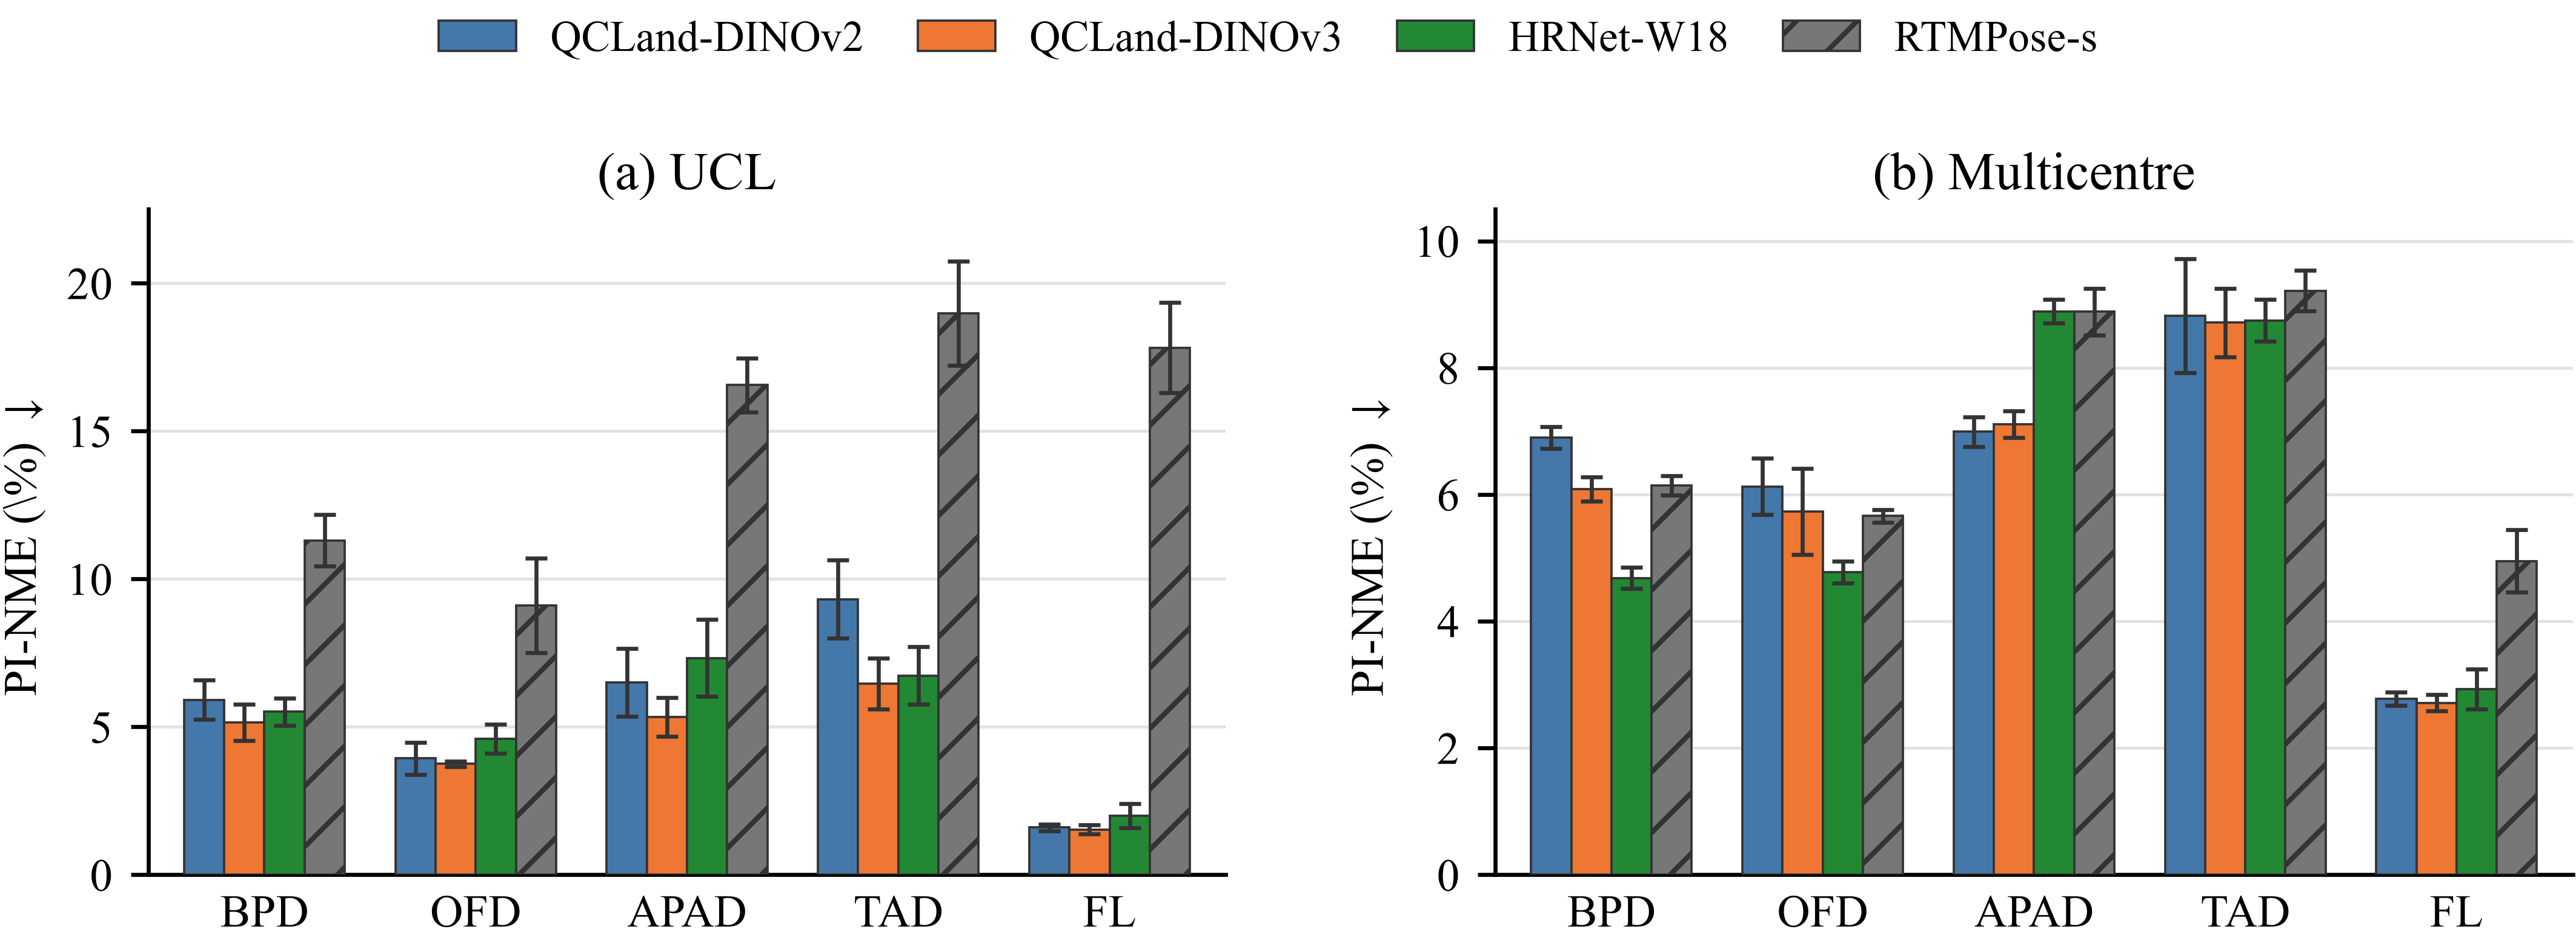
\includegraphics[width=\textwidth]
    {figures/final_four_model_comparison.png}
  \caption{Final four-model comparison across the UCL and Multicentre
    evaluation settings. Bars show five-seed mean PI-NME and error
    bars show the seed-level sample standard deviation for each fetal
    measurement. Lower PI-NME indicates better localisation
    performance. The two panels use different vertical scales for
    readability.}
  \label{fig:four-model-bar}
\end{figure}

The eight-of-ten ranking provides a concise descriptive summary of
QCLand's competitiveness, but it does not imply that every numerical
advantage is statistically supported. The paired analysis therefore
distinguishes descriptive rankings from confirmed differences.


\subsection{Effect of Backbone Choice}
\label{sec:results-backbone}

QCLand-DINOv3 has a lower mean PI-NME than QCLand-DINOv2 in nine of
the ten evaluation settings. The only reversal is Multicentre APAD,
where DINOv2 records 6.99\% and DINOv3 7.11\%. The directional
pattern therefore consistently favours DINOv3 at the descriptive
level.

Inferential support is more limited. None of the five UCL
DINOv2--DINOv3 contrasts reaches Holm-60 Wilcoxon significance.
APAD and TAD have bootstrap intervals that exclude zero without
corresponding Wilcoxon support and are therefore treated as
test-discordant rather than confirmed effects. On Multicentre, BPD
and OFD are supported by both analyses ($p<0.001$), whereas the other
three measurements are not.

The evidence therefore favours DINOv3 descriptively across most
settings but does not support a blanket claim that the newer backbone
is superior for every fetal landmark-localisation task.


\subsection{Comparison with HRNet-W18 and RTMPose-s}
\label{sec:results-baselines}

The paired contrasts are reported in
\Cref{tab:ucl-paired,tab:multicentre-paired}. The discussion below
focuses on the main patterns rather than repeating every numerical
entry.

\paragraph{QCLand versus HRNet-W18.}
On UCL, QCLand and HRNet-W18 are largely comparable. The only
contrast supported by both analyses is TAD with QCLand-DINOv2, for
which QCLand performs worse than HRNet-W18. QCLand-DINOv3 on the
same measurement is statistically indistinguishable from HRNet-W18.
Both QCLand variants show Wilcoxon-supported advantages on FL, but
their bootstrap intervals cross zero.

The Multicentre results are more anatomy-dependent. HRNet-W18
outperforms both QCLand variants on BPD and OFD with agreement between
the bootstrap and Wilcoxon analyses. QCLand, by contrast, outperforms
HRNet-W18 on APAD for both backbones. FL again provides rank-based
support for QCLand without bootstrap confirmation, while TAD shows no
supported difference. Neither architecture therefore dominates
uniformly across anatomical measurements.

\paragraph{QCLand versus RTMPose-s.}
On UCL, both QCLand backbones outperform RTMPose-s on every
measurement, with particularly large differences for FL and the
abdominal measurements.

RTMPose-s is more competitive on Multicentre. QCLand significantly
outperforms it on APAD and FL, while TAD shows no supported
difference. On BPD and OFD, QCLand-DINOv2 performs worse than
RTMPose-s, whereas the DINOv3 backbone substantially narrows this gap.
The evidence therefore does not support a universal advantage of
heatmap-based spatial decoding over coordinate classification.

\begin{table}[htbp]
  \centering
  \caption{UCL paired contrasts (QCLand vs.\ baselines). Differences
    are in percentage points; negative values favour QCLand.}
  \label{tab:ucl-paired}
  \footnotesize
  \setlength{\tabcolsep}{4pt}
  \renewcommand{\arraystretch}{0.92}
  \begin{tabular}{llrrl}
    \toprule
    Task & Contrast & Diff., pp & 95\% CI & Holm-60 $p$ \\
    \midrule
    \multirow{4}{*}{BPD}
      & DINOv2 $-$ HRNet-W18   & 0.41  & [$-$0.98, 1.67]       & 0.081 \\
      & DINOv2 $-$ RTMPose-s   & $-$5.39 & [$-$7.63, $-$3.34] & $<$0.001 \\
      & DINOv3 $-$ HRNet-W18   & $-$0.37 & [$-$1.77, 0.76]    & 0.219 \\
      & DINOv3 $-$ RTMPose-s   & $-$6.16 & [$-$8.51, $-$4.00] & $<$0.001 \\
    \cmidrule(lr){2-5}
    \multirow{4}{*}{OFD}
      & DINOv2 $-$ HRNet-W18   & $-$0.65 & [$-$1.78, 0.16]    & 0.861 \\
      & DINOv2 $-$ RTMPose-s   & $-$5.18 & [$-$7.25, $-$3.37] & $<$0.001 \\
      & DINOv3 $-$ HRNet-W18   & $-$0.84 & [$-$2.19, 0.07]    & 1.000 \\
      & DINOv3 $-$ RTMPose-s   & $-$5.36 & [$-$7.50, $-$3.49] & $<$0.001 \\
    \cmidrule(lr){2-5}
    \multirow{4}{*}{APAD}
      & DINOv2 $-$ HRNet-W18   & $-$0.83 & [$-$3.12, 1.25]    & 1.000 \\
      & DINOv2 $-$ RTMPose-s   & $-$10.06 & [$-$13.35, $-$7.23] & $<$0.001 \\
      & DINOv3 $-$ HRNet-W18   & $-$1.99 & [$-$4.80, 0.51]    & 1.000 \\
      & DINOv3 $-$ RTMPose-s   & $-$11.22 & [$-$14.94, $-$8.16] & $<$0.001 \\
    \cmidrule(lr){2-5}
    \multirow{4}{*}{TAD}
      & DINOv2 $-$ HRNet-W18   & 2.58  & [0.42, 5.16]          & 0.035 \\
      & DINOv2 $-$ RTMPose-s   & $-$9.66 & [$-$14.99, $-$4.93] & 0.005 \\
      & DINOv3 $-$ HRNet-W18   & $-$0.27 & [$-$2.80, 2.20]    & 0.474 \\
      & DINOv3 $-$ RTMPose-s   & $-$12.51 & [$-$16.51, $-$8.99] & $<$0.001 \\
    \cmidrule(lr){2-5}
    \multirow{4}{*}{FL}
      & DINOv2 $-$ HRNet-W18   & $-$0.39 & [$-$2.11, 0.55]    & $<$0.001 \\
      & DINOv2 $-$ RTMPose-s   & $-$16.22 & [$-$26.67, $-$8.91] & $<$0.001 \\
      & DINOv3 $-$ HRNet-W18   & $-$0.46 & [$-$2.20, 0.51]    & 0.004 \\
      & DINOv3 $-$ RTMPose-s   & $-$16.29 & [$-$26.65, $-$9.07] & $<$0.001 \\
    \bottomrule
  \end{tabular}
  \par\smallskip
  {\footnotesize Intervals are 95\% paired-bootstrap CIs; $p$ is
    globally Holm-60 adjusted. DINOv2--DINOv3 and HRNet--RTMPose-s
    contrasts are available in the frozen statistical records.}
\end{table}

\begin{table}[htbp]
  \centering
  \caption{Multicentre paired contrasts (QCLand vs.\ baselines).
    Differences are in percentage points; negative values favour
    QCLand.}
  \label{tab:multicentre-paired}
  \footnotesize
  \setlength{\tabcolsep}{4pt}
  \renewcommand{\arraystretch}{0.92}
  \begin{tabular}{llrrl}
    \toprule
    Task & Contrast & Diff., pp & 95\% CI & Holm-60 $p$ \\
    \midrule
    \multirow{4}{*}{BPD}
      & DINOv2 $-$ HRNet-W18   & 2.21  & [1.90, 2.52]          & $<$0.001 \\
      & DINOv2 $-$ RTMPose-s   & 0.75  & [0.41, 1.08]          & $<$0.001 \\
      & DINOv3 $-$ HRNet-W18   & 1.40  & [1.13, 1.67]          & $<$0.001 \\
      & DINOv3 $-$ RTMPose-s   & $-$0.06 & [$-$0.39, 0.24]    & 0.016 \\
    \cmidrule(lr){2-5}
    \multirow{4}{*}{OFD}
      & DINOv2 $-$ HRNet-W18   & 1.35  & [0.98, 1.75]          & $<$0.001 \\
      & DINOv2 $-$ RTMPose-s   & 0.47  & [0.12, 0.82]          & $<$0.001 \\
      & DINOv3 $-$ HRNet-W18   & 0.96  & [0.63, 1.30]          & $<$0.001 \\
      & DINOv3 $-$ RTMPose-s   & 0.07  & [$-$0.23, 0.38]      & 1.000 \\
    \cmidrule(lr){2-5}
    \multirow{4}{*}{APAD}
      & DINOv2 $-$ HRNet-W18   & $-$1.90 & [$-$2.71, $-$1.15] & $<$0.001 \\
      & DINOv2 $-$ RTMPose-s   & $-$1.89 & [$-$2.91, $-$1.03] & $<$0.001 \\
      & DINOv3 $-$ HRNet-W18   & $-$1.78 & [$-$2.53, $-$1.08] & 0.005 \\
      & DINOv3 $-$ RTMPose-s   & $-$1.78 & [$-$2.62, $-$1.02] & $<$0.001 \\
    \cmidrule(lr){2-5}
    \multirow{4}{*}{TAD}
      & DINOv2 $-$ HRNet-W18   & 0.07  & [$-$0.74, 0.89]       & 1.000 \\
      & DINOv2 $-$ RTMPose-s   & $-$0.40 & [$-$1.75, 0.76]    & 1.000 \\
      & DINOv3 $-$ HRNet-W18   & $-$0.04 & [$-$0.69, 0.63]    & 1.000 \\
      & DINOv3 $-$ RTMPose-s   & $-$0.50 & [$-$1.96, 0.66]    & 1.000 \\
    \cmidrule(lr){2-5}
    \multirow{4}{*}{FL}
      & DINOv2 $-$ HRNet-W18   & $-$0.15 & [$-$0.74, 0.30]    & $<$0.001 \\
      & DINOv2 $-$ RTMPose-s   & $-$2.17 & [$-$5.00, $-$0.59] & $<$0.001 \\
      & DINOv3 $-$ HRNet-W18   & $-$0.22 & [$-$0.82, 0.23]    & $<$0.001 \\
      & DINOv3 $-$ RTMPose-s   & $-$2.24 & [$-$5.16, $-$0.56] & $<$0.001 \\
    \bottomrule
  \end{tabular}
  \par\smallskip
  {\footnotesize Intervals are 95\% paired-bootstrap CIs; $p$ is
    globally Holm-60 adjusted. DINOv2--DINOv3 and HRNet--RTMPose-s
    contrasts are available in the frozen statistical records.}
\end{table}


\subsection{Interpretation of the Comparative Results}
\label{sec:discussion-comparative}
\label{sec:discussion-significance}

Taken together, the comparative evidence supports the central claim
behind RQ1 and RQ3: query-conditioned foundation-model
representations can be adapted effectively to precise fetal landmark
localisation, but their advantage is not invariant to anatomy or
dataset setting.

The clearest distinction from HRNet-W18 lies in the anatomical
pattern. QCLand is strongest on the abdominal measurements and remains
competitive on FL, whereas HRNet-W18 retains a clear advantage on the
Multicentre head measurements. This suggests that the value of
pretrained transformer representations and query-conditioned spatial
decoding depends on the geometry and appearance characteristics of the
target measurement rather than uniformly replacing a convolutional
landmark architecture.

RTMPose-s provides a complementary comparison. Its poor UCL
performance shows that a modern coordinate-classification formulation
does not automatically transfer well to these relatively small fetal
datasets. Its stronger Multicentre performance, particularly on the
head measurements, nevertheless prevents a general conclusion that
dense heatmap decoding is inherently superior to coordinate
classification.

The DINOv2--DINOv3 comparison follows the same pattern of qualified
evidence. DINOv3 records the lower mean in nine of ten settings, but
paired support is concentrated on Multicentre BPD and OFD. The larger
Multicentre samples may make smaller differences easier to detect, but
the present experiments do not include a matched subsampling analysis
capable of separating statistical power from genuinely
dataset-dependent backbone behaviour.


% =================================================================
% 5.2 Results of Ablation Study
% =================================================================

\section{Results of Ablation Study}
\label{sec:results-development}
\label{sec:results-track-a}

The BPD experiments trace the development of the adopted QCLand
configuration and address RQ2. The study includes both controlled
component comparisons and sequential development steps. It is
therefore interpreted as a staged ablation study rather than a fully
factorial decomposition of every component. The target-width
experiment is a single-seed exploratory screen; the subsequent
controlled comparisons use the five predefined seeds unless stated
otherwise.


\subsection{Target Width and Objective Selection}
\label{sec:results-bpd-sigma}
\label{sec:results-bpd-loss}

An initial single-seed experiment (seed 2024) using the original
dot-product readout showed that increasing the Gaussian target width
from $\sigma=1$ to $\sigma=4$ reduced PI-NME from 149.89\% to
50.46\%. This exploratory result motivated the use of $\sigma=4$ in
the subsequent experiments and is not treated as a formal five-seed
comparison.

The training objective was then examined under a controlled five-seed
design while retaining the dot-product readout.

\begin{table}[htbp]
  \centering
  \caption{BPD loss screening, dot-product readout, five-seed
    final-checkpoint PI-NME, mean $\pm$ sample SD, $n=49$.}
  \label{tab:bpd-loss}
  \begin{tabular}{@{}lr@{}}
    \toprule
    Loss & PI-NME \\
    \midrule
    Plain heatmap MSE
      & 36.65 $\pm$ 17.28\% \\
    Weighted heatmap MSE
      & 13.75 $\pm$ 2.90\% \\
    Hybrid (weighted MSE + coordinate L1)
      & 11.23 $\pm$ 2.06\% \\
    \bottomrule
  \end{tabular}
\end{table}

Plain heatmap MSE produced both the highest error and the greatest
seed-to-seed variability. Peak reweighting substantially reduced both,
and adding coordinate supervision produced a further reduction. The
hybrid objective was therefore adopted for all subsequent
experiments.


\subsection{Contribution of DeconvHeadV2 and Feature Fusion}
\label{sec:results-bpd-ablation}

The staged architecture chain is summarised in
\Cref{tab:bpd-progression,fig:bpd-development}. All four
configurations use the hybrid objective, the same five seeds, and the
same PI-NME evaluation.

\begin{table}[htbp]
  \centering
  \caption{BPD architecture development chain, five-seed
    final-checkpoint PI-NME, mean $\pm$ sample SD, $n=49$.}
  \label{tab:bpd-progression}
  \begin{tabular}{@{}lr@{}}
    \toprule
    Configuration & PI-NME \\
    \midrule
    Dot-product readout (baseline)
      & 11.23 $\pm$ 2.06\% \\
    DeconvHeadV2
      & 8.12 $\pm$ 1.42\% \\
    \quad + multi-depth fusion
      & 9.00 $\pm$ 2.20\% \\
    \quad + pixel-centre alignment
      & 8.96 $\pm$ 2.30\% \\
    \bottomrule
  \end{tabular}
\end{table}

\begin{figure}[p]
  \centering
  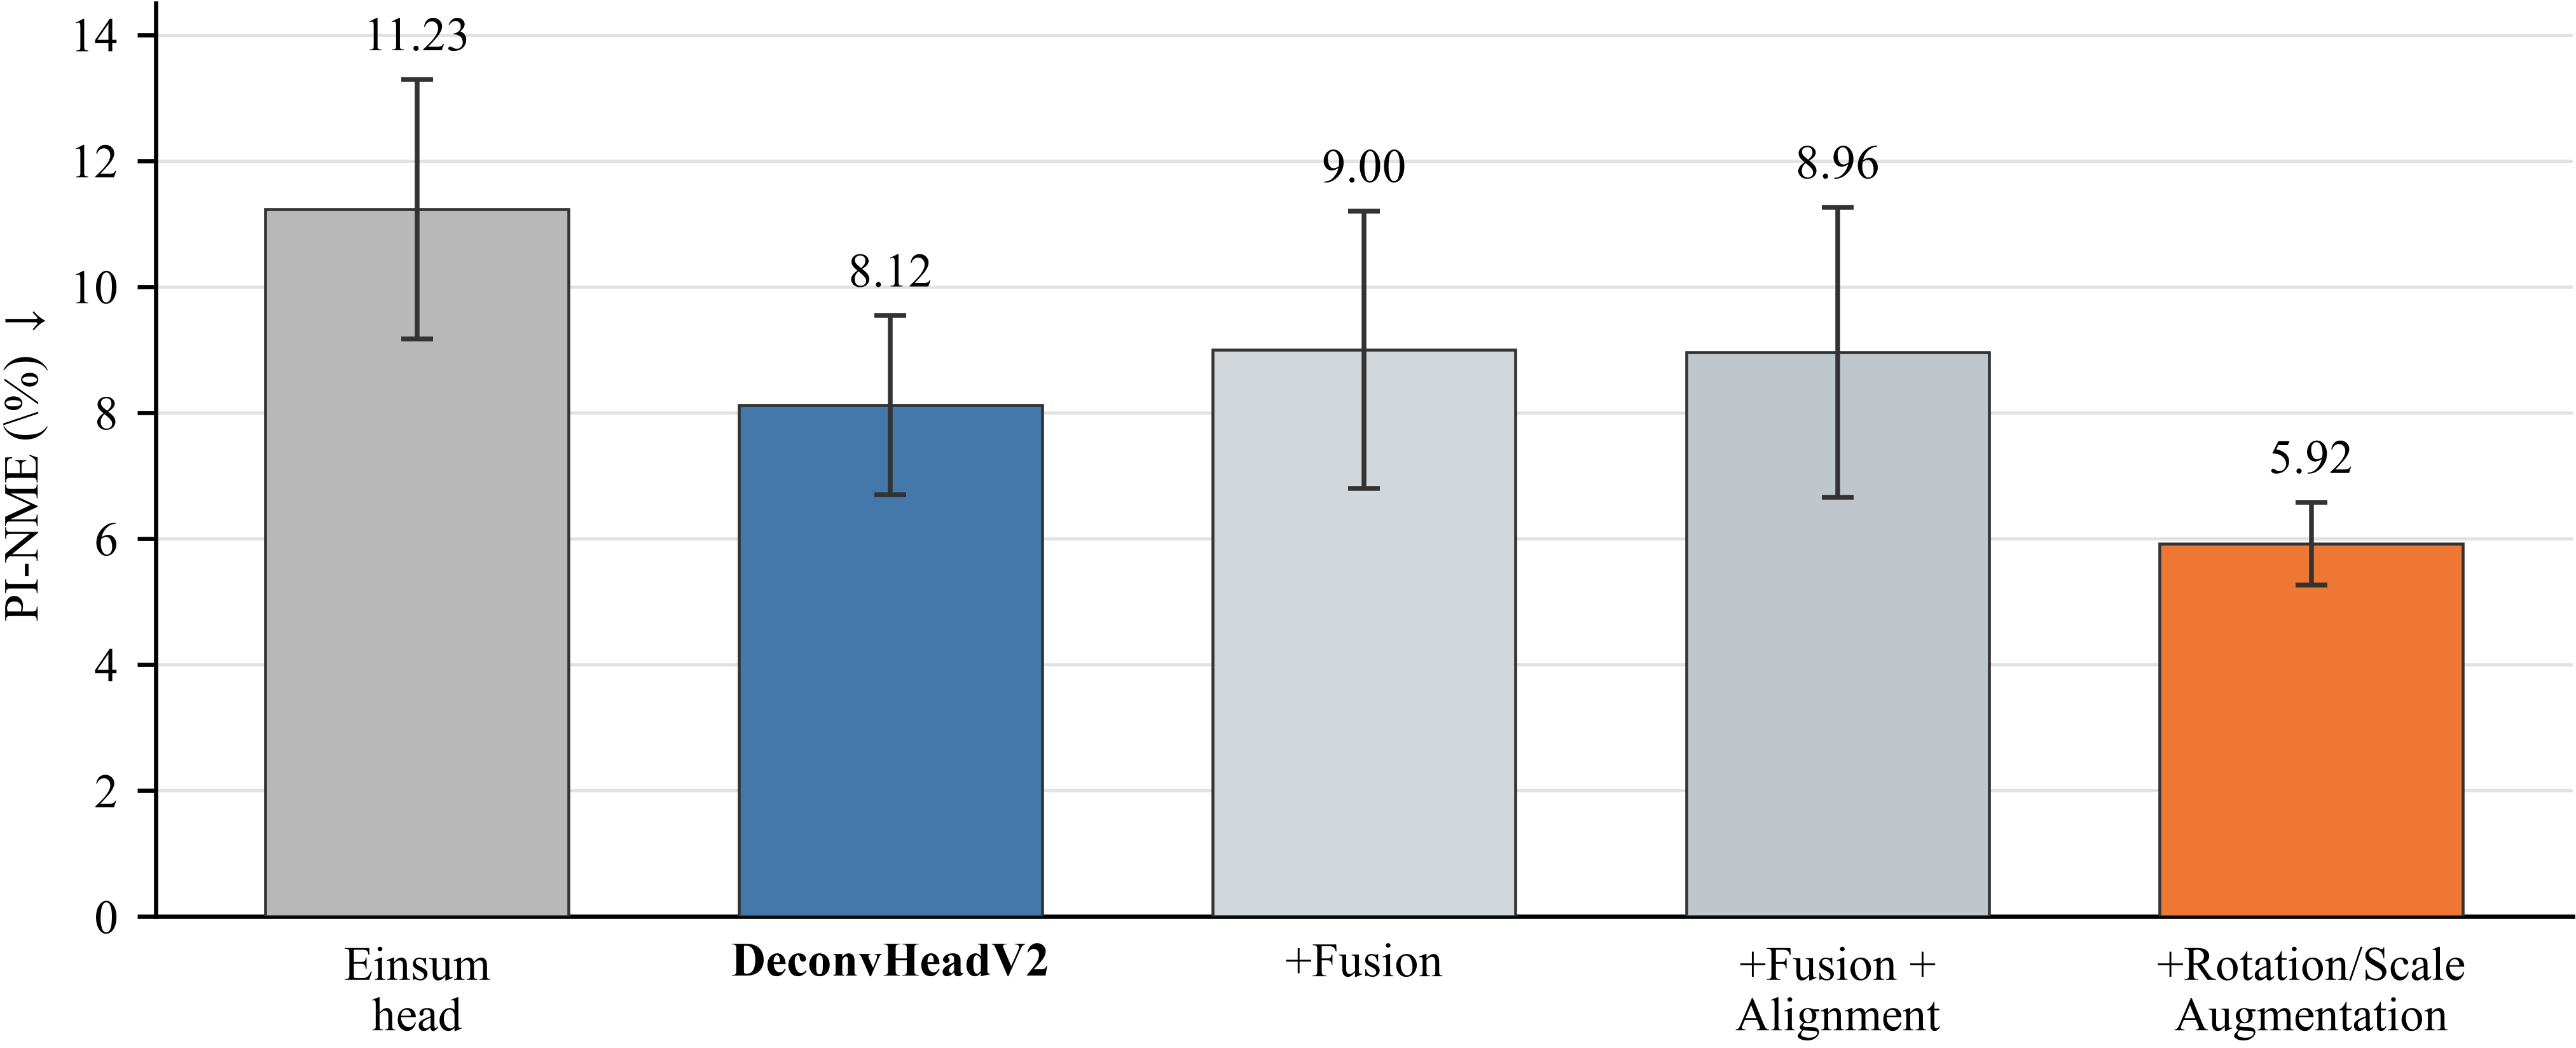
\includegraphics[width=0.95\textwidth]
    {figures/bpd_staged_development.png}
  \caption{Staged BPD ablation results. Bars show five-seed mean
    PI-NME and error bars show seed-level sample SD. The sequence
    represents model development rather than a factorial ablation.}
  \label{fig:bpd-development}

  \vspace{0.8em}

  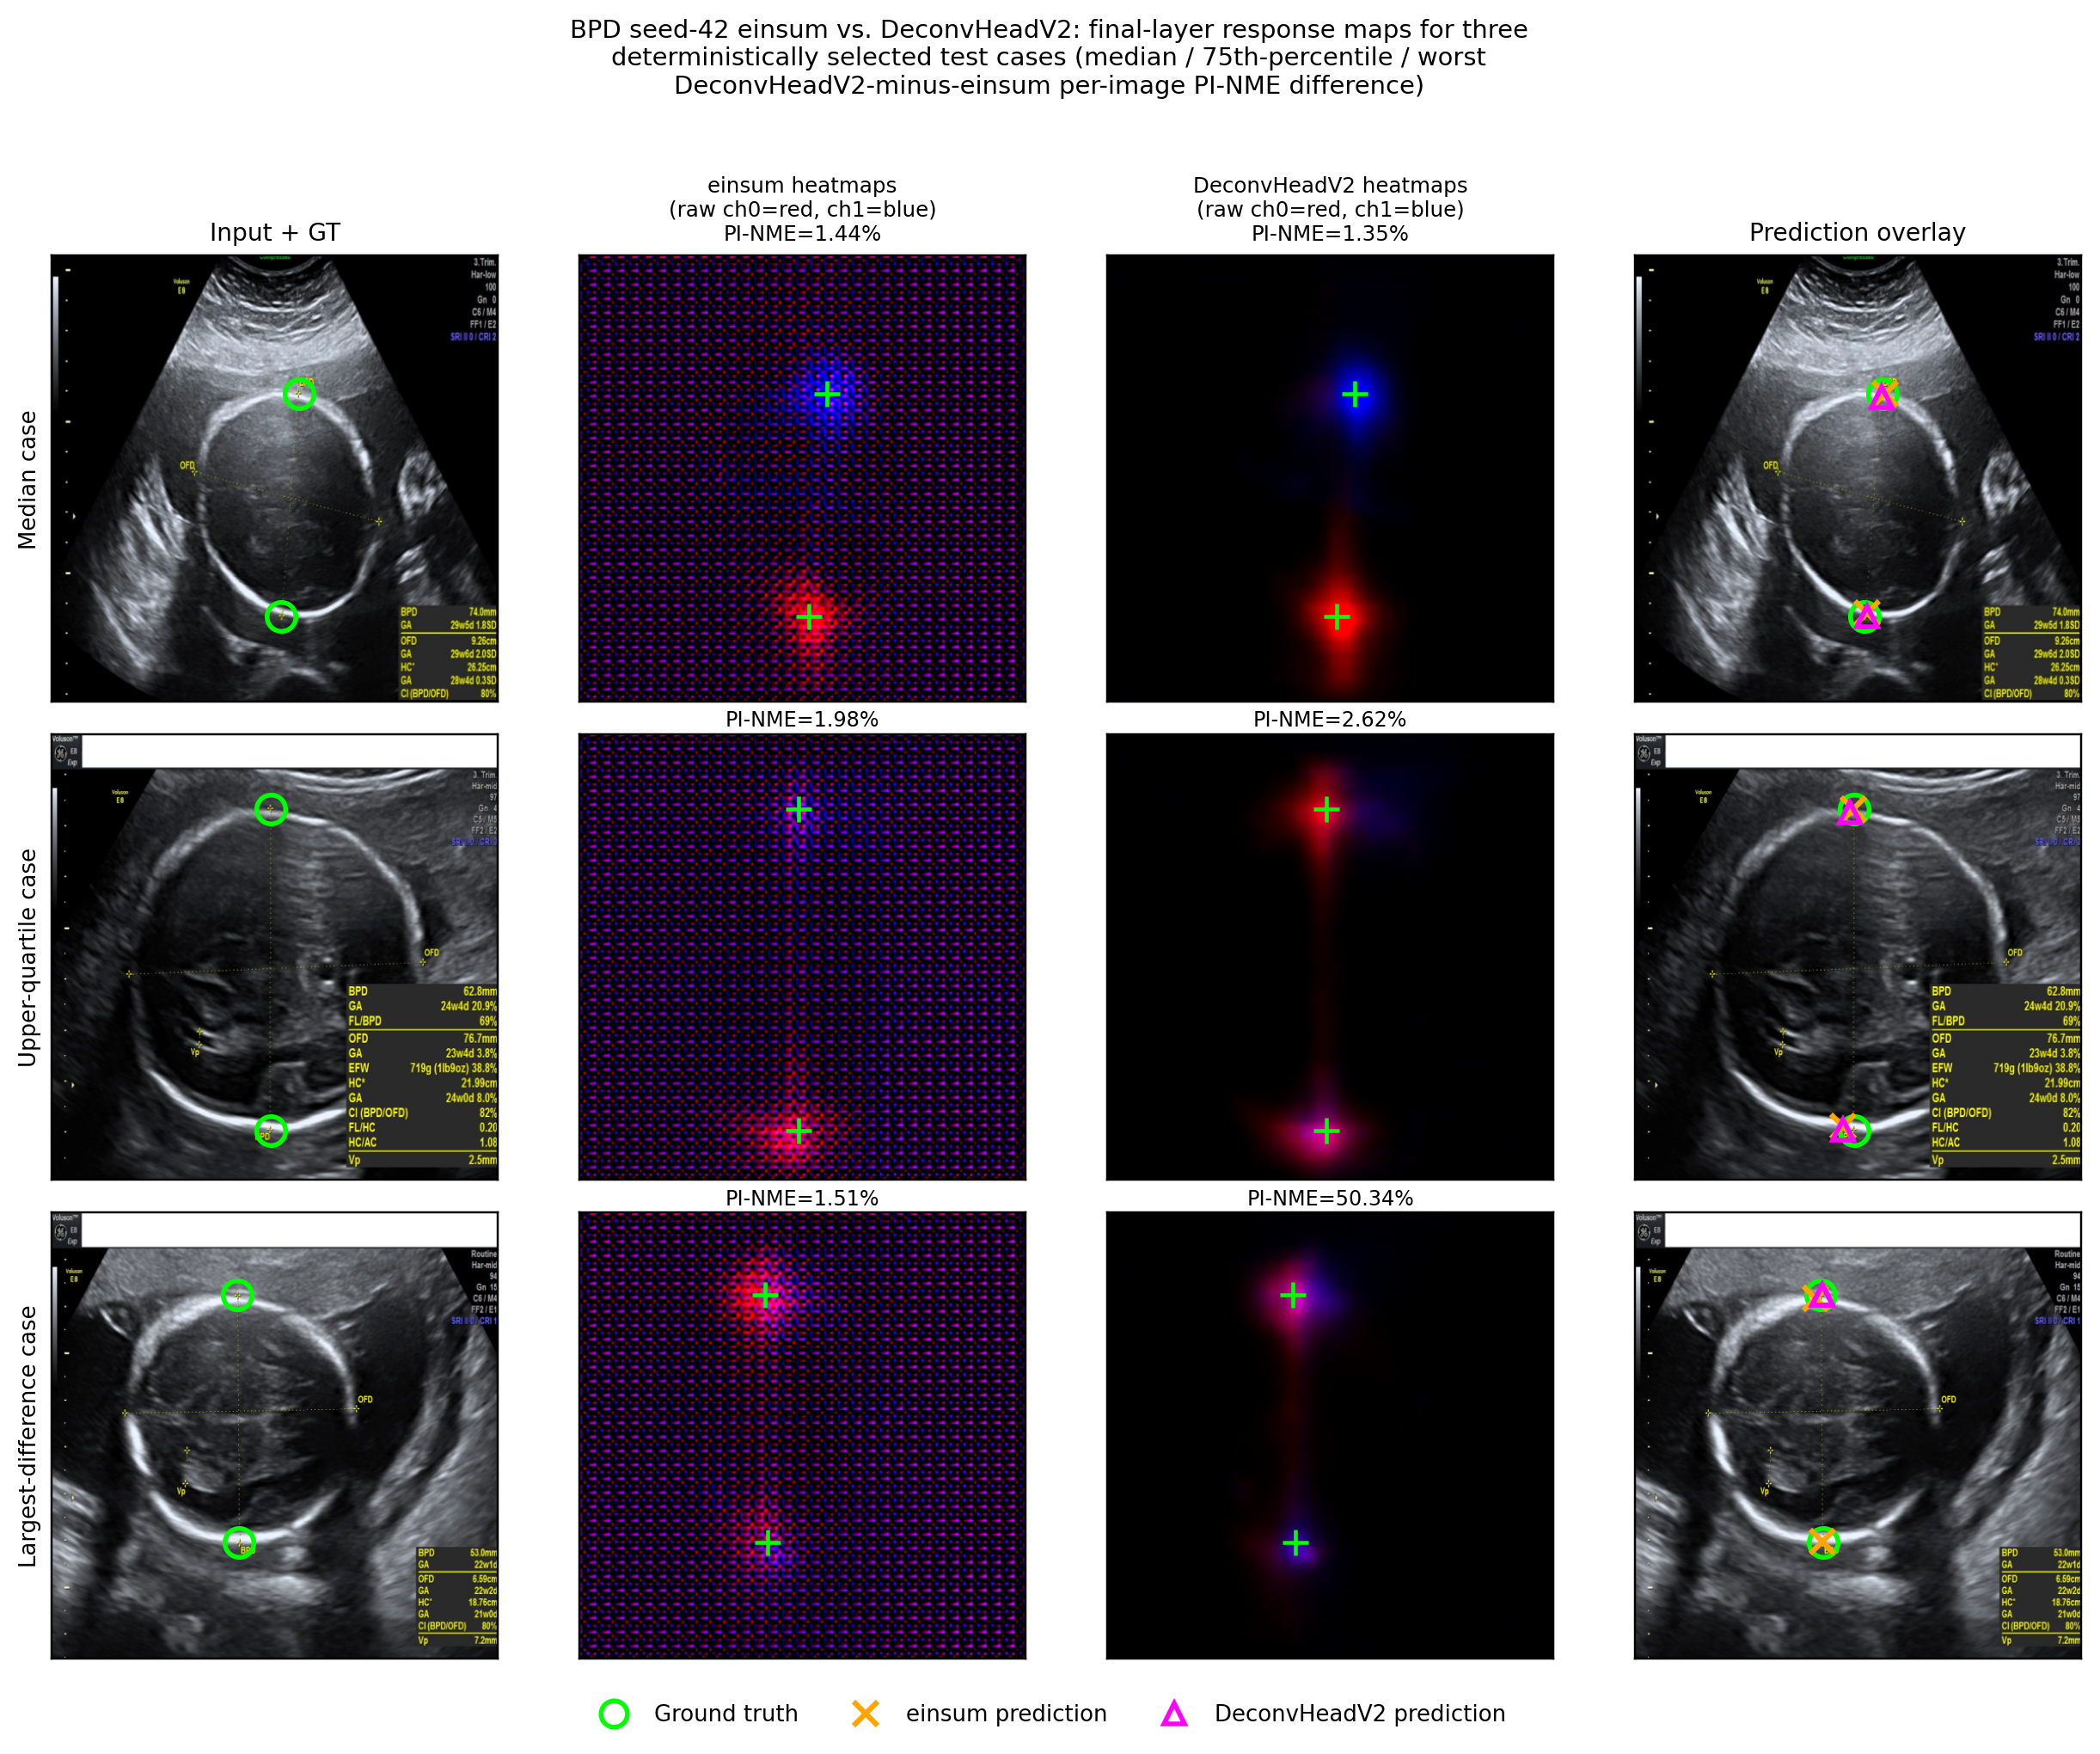
\includegraphics[width=0.95\textwidth]
    {figures/bpd_einsum_deconvheadv2_heatmaps.png}
  \caption[Qualitative readout comparison]{Qualitative comparison of
    the dot-product readout and DeconvHeadV2 on three deterministically
    selected BPD cases (seed 42). Heatmaps show the raw query channels
    (channel 0 red, channel 1 blue); green, orange, and magenta markers
    denote ground truth, dot-product predictions, and DeconvHeadV2
    predictions, respectively. The examples are illustrative rather
    than a statistical sample.}
  \label{fig:einsum-deconvheadv2-heatmaps}
\end{figure}

DeconvHeadV2 produces the largest observed architectural improvement,
reducing PI-NME from $11.23\pm2.06\%$ to $8.12\pm1.42\%$. This is
consistent with its intended role: replacing an independent
per-location dot-product readout with a query-conditioned spatial
decoder capable of local spatial mixing.

Adding multi-depth feature fusion does not further reduce the mean in
the unaugmented chain ($8.12\%\rightarrow9.00\%$), while adding
pixel-centre alignment produces only a small numerical change
($9.00\%\rightarrow8.96\%$). No paired significance tests were
performed between these sequential architecture rungs, so these
differences are interpreted descriptively.

The qualitative comparison provides a complementary view of the
decoder change. In two of the three deterministically selected cases,
DeconvHeadV2 produces visibly more concentrated responses than the
dot-product readout. The remaining case shows both query channels
responding to the same spatial peak, illustrating that the aggregate
improvement does not eliminate all image-level failure modes.


\subsection{Effect of Rotation-and-Scale Augmentation}
\label{sec:results-augmentation}

Rotation-and-scale augmentation is associated with the largest
subsequent reduction in the complete development chain. The
unaugmented complete configuration records $8.96\pm2.30\%$, compared
with $5.92\pm0.66\%$ for the corresponding augmented
QCLand-DINOv2 configuration. The change is accompanied by a
substantial reduction in run-to-run variability.

Because the sequential comparison cannot determine whether this
improvement arises from augmentation alone or from its interaction
with fusion and alignment, a targeted matched follow-up compares
augmented DeconvHeadV2 alone with the complete augmented
configuration.

\begin{table}[htbp]
  \centering
  \caption{BPD augmented-configuration comparison, five-seed
    final-checkpoint PI-NME, mean $\pm$ sample SD, $n=49$.}
  \label{tab:bpd-augmented}
  \begin{tabular}{@{}lr@{}}
    \toprule
    Configuration & PI-NME \\
    \midrule
    DeconvHeadV2 + augmentation
      & 6.30 $\pm$ 0.67\% \\
    DeconvHeadV2 + fusion + alignment + augmentation
      & 5.92 $\pm$ 0.66\% \\
    \bottomrule
  \end{tabular}
\end{table}

The complete configuration has a 0.38 percentage-point lower mean.
The 20{,}000-resample paired-bootstrap confidence interval crosses
zero ($-0.48$ to $+1.28$), whereas the Pratt--Wilcoxon test rejects
its null hypothesis ($p=0.0078$). The bootstrap therefore does not
confirm a non-zero mean difference, while the rank-based analysis
supports a distributional shift. Because fusion and pixel-centre
alignment change together in this contrast, their individual
contributions remain unresolved.


\subsection{Input-Resolution Sensitivity}
\label{sec:results-resolution}

A matched five-seed comparison between $256\times256$ and
$512\times512$ input resolution was conducted using the complete
augmented QCLand-DINOv2 configuration. Heatmap resolution remained
fixed at $64\times64$. The higher-resolution configuration produces a
numerically lower mean and smaller run-to-run spread
($6.61\pm0.91\%$ versus $7.30\pm1.50\%$). No paired significance
test was conducted, so the comparison remains descriptive. The
$512\times512$ result in this experiment is an independent
matched-control run rather than the QCLand-DINOv2 value in the final
four-model table.


\subsection{Interpretation of the Ablation Study}
\label{sec:discussion-development}
\label{sec:discussion-components}

The ablation evidence identifies the spatial decoder as the most
consequential architectural change. DeconvHeadV2 modifies several
elements simultaneously---FiLM conditioning, GroupNorm,
convolutional capacity, and initialisation---so the improvement should
be attributed to the module as a whole rather than to any one of its
internal components. Its strong effect nevertheless supports the
central architectural motivation of QCLand: pretrained query
representations require an explicit spatial readout capable of
transforming them into precise landmark responses.

The evidence for multi-depth fusion and pixel-centre alignment is more
limited. Neither improves the unaugmented sequential chain, and their
combined contribution under augmentation produces discordant bootstrap
and Wilcoxon conclusions. Their independent effects therefore cannot
be established from the present experiments.

Augmentation has a clearer empirical role. The reduction in both mean
PI-NME and run-to-run variability suggests that exposing the model to
rotation and scale variation materially improves the robustness of the
adopted configuration on BPD. The current design, however, does not
isolate the mechanism responsible for that gain.

The development evidence is also specific to BPD. The other four
measurements evaluate the adopted configuration as a complete pipeline
rather than repeating the full ablation sequence. Their results
therefore demonstrate the applicability of the final recipe across
measurements, not the independent transfer of every component.


% =================================================================
% 5.3 Variation Across Measurements and Dataset Settings
% =================================================================

\section{Variation Across Measurements and Dataset Settings}
\label{sec:discussion-variation}
\label{sec:discussion-multicentre-vs-ucl}

The changing model ranking across measurements and datasets suggests
that several factors interact with architecture and backbone choice.
The present design does not isolate these factors, but three
observations provide plausible directions for interpretation.

\textbf{Data scale and statistical power.}
The Multicentre training pools are substantially larger than their UCL
counterparts. This may influence both optimisation stability and the
ability of paired statistical tests to detect relatively small
differences. HRNet-W18 also shows substantially tighter seed-level
variation on Multicentre. Dataset composition changes at the same
time, however, so these differences cannot be attributed to sample
size alone.

\textbf{Measurement geometry and landmark orientation.}
QCLand uses left-to-right landmark assignment during training. For
landmark pairs with little horizontal separation, small geometric
perturbations can reverse this ordering and change the query
assignment. HRNet-W18's DOD formulation instead imposes ordering
through a learned measurement-specific direction. This provides one
possible explanation for anatomy-dependent differences, but no
per-image landmark-angle analysis was conducted, so the aggregate
results cannot establish the mechanism.

\textbf{Domain and device diversity.}
The pooled Multicentre benchmark introduces additional variation in
clinical site, ultrasound device, and source-dataset composition.
QCLand does not obtain a uniform advantage under this broader
variation, indicating that large-scale self-supervised pretraining
alone does not guarantee superior performance across all source and
measurement combinations. Anatomy, training-set size, and source
composition change simultaneously and cannot be separated by the
present experiments.


% =================================================================
% 5.4 Limitations
% =================================================================

\section{Limitations}
\label{sec:discussion-limitations}


\subsection{Dataset Scope}

The Multicentre benchmark is not centre-held-out: its released
partition contains data from the constituent clinical sources on both
sides of the Train/Test split. Its results should therefore be
interpreted as performance on a pooled multi-site benchmark rather
than as a direct test of transfer to an unseen clinical centre.

UCL is also one of the constituent sources of the pooled Multicentre
release, so the UCL and Multicentre experiments should not be regarded
as fully independent replications of the same finding.

The paired bootstrap resamples images independently and does not
explicitly model correlations among repeated frames. The resulting
confidence intervals therefore characterise image-level uncertainty
under the adopted evaluation protocol rather than a hierarchical
subject-level sampling process.


\subsection{Evaluation and Comparison}
\label{sec:discussion-limitations-comparison}
\label{sec:discussion-limitations-resolution}
\label{sec:discussion-limitations-filtering}

The four-model comparison harmonises input resolution, external
metric, common evaluation images, and training seeds, but the models
retain different training procedures. QCLand uses validation-based
termination with a terminal-state checkpoint, HRNet-W18 follows its
upstream procedure, and RTMPose-s trains for a fixed number of epochs.
The comparison therefore evaluates complete methods under harmonised
external conditions rather than isolating architecture alone.

The upstream HRNet-W18 loader excludes rows with negative or missing
landmark coordinates, slightly reducing the common image subset for
some Multicentre measurements. All models are evaluated on the
resulting intersection, but the eligibility rule originates from the
baseline implementation.

Published BiometryNet numbers are used only for contextual reference.
Their training procedure, input resolution, and complete evaluation
implementation are not protocol-matched to the local reproduction.


\subsection{Method Development and Landmark Assignment}
\label{sec:discussion-limitations-method}
\label{sec:discussion-limitations-valset}

The relatively small UCL internal validation sets make
validation-based termination potentially noisy. Although QCLand
reports the terminal state rather than selecting the best validation
checkpoint, the stopping epoch remains influenced by this validation
sample.

The left-to-right landmark assignment used during training can become
unstable when a landmark pair has little horizontal separation.
PI-NME removes the corresponding ordering ambiguity during evaluation,
but it does not change the query-specific supervision used in
training. A direct assessment would require per-image analysis of
landmark orientation and localisation error, which was not undertaken
in the present study.

The BPD ablation sequence is staged rather than factorial, so the
effect of a modification depends on the configuration that precedes
it. Fusion and pixel-centre alignment are also varied together in the
augmented follow-up and therefore cannot be individually isolated.
The analysis consequently identifies the most consequential complete
changes rather than estimating an independent causal contribution for
every component.


% =================================================================
% 5.5 Implications and Future Directions
% =================================================================

\section{Implications and Future Directions}
\label{sec:discussion-implications}
\label{sec:discussion-eomt-suitability}

Taken together, the results show that self-supervised vision
foundation models provide an effective basis for precise fetal
landmark localisation when combined with landmark-query interaction
and an appropriate spatial decoder. A QCLand variant records the
lowest mean error in eight of ten settings, while the ablation study
identifies DeconvHeadV2 as the most consequential architectural
modification during model development.

The anatomy-dependent ranking between QCLand and HRNet-W18 is equally
important. Neither query-conditioned foundation-model adaptation nor
a purpose-built convolutional landmark architecture is universally
superior. The Multicentre head measurements remain the clearest case
where the convolutional baseline retains an advantage, motivating
targeted analysis of measurement geometry and representation choice.

A per-image landmark-orientation analysis would directly test whether
training-time landmark assignment contributes to the observed
anatomical differences. If supported, orientation-aware
canonicalisation or permutation-aware training objectives would be
natural extensions.

A controlled Multicentre subsampling study would also help distinguish
effects of training-set size from those of source diversity and
measurement geometry. Finally, extending the ablation study to at
least one non-head measurement would test whether the strong
DeconvHeadV2 result and the more uncertain fusion/alignment effects
generalise beyond the BPD development task.


% =================================================================
% 5.6 Main Findings
% =================================================================

\section{Main Findings}
\label{sec:results-summary}
\label{sec:results-comparative-summary}

Two conclusions emerge from the combined results and discussion.
First, QCLand is competitive with established landmark-localisation
methods across the evaluated fetal measurements: a QCLand variant
records the lowest mean PI-NME in eight of ten settings, although the
relative advantage is anatomy- and dataset-dependent. Second, the BPD
ablation study identifies DeconvHeadV2 as the architectural change
associated with the largest observed improvement, while the
independent contributions of multi-depth fusion and pixel-centre
alignment remain less certain.

The evidence therefore supports query-conditioned foundation-model
adaptation as a viable approach to precise fetal landmark localisation
without implying universal superiority over purpose-built
alternatives. The following chapter consolidates these findings into
the thesis conclusions and outlines the most important directions for
further validation and development.

\chapter{Conclusion}
\label{chap:conclusion}


% =================================================================
% 6.1 Conclusions
% =================================================================

\section{Conclusions}
\label{sec:conclusion-summary}

This thesis investigated whether self-supervised vision foundation
models can be adapted for precise fetal biometry landmark
localisation. To bridge the gap between general-purpose visual
representations and the spatially precise, measurement-specific
predictions required for fetal biometry, it introduced QCLand, a
query-conditioned landmark-localisation framework that combines
learned landmark queries with pretrained DINOv2 and DINOv3 backbones
and a new spatial decoding head, DeconvHeadV2.

The final comparison provides evidence that QCLand can be adapted
effectively to this task. A QCLand variant records the lowest mean
PI-NME in eight of the ten dataset--measurement settings, with
QCLand-DINOv3 achieving the lowest mean on all five UCL
measurements. These results support query-conditioned
foundation-model adaptation as a viable approach to precise fetal
landmark localisation within the evaluated benchmark settings.

The BPD ablation study further clarifies where the observed
performance gains arise. DeconvHeadV2 produces the largest reduction
in localisation error among the evaluated architectural
modifications. Rotation-and-scale augmentation is associated with a
further substantial reduction in mean error and lower run-to-run
variability. By contrast, the independent contributions of
multi-depth feature fusion and pixel-centre alignment remain
unresolved by the sequential experimental design.

Performance nevertheless varies across anatomy, backbone, and dataset
setting. DINOv3 is descriptively stronger than DINOv2 in most
comparisons, but paired statistical support is confined to two
Multicentre measurements. The QCLand--HRNet-W18 ranking is similarly
anatomy-dependent: QCLand shows its clearest confirmed advantage on
Multicentre APAD, whereas HRNet-W18 retains a clear advantage on the
Multicentre head measurements. RTMPose-s is consistently weaker on
UCL but remains competitive in several Multicentre settings.

QCLand is therefore competitive across the evaluated fetal
landmark-localisation tasks, but its advantages are conditional rather
than universal. The results support the effectiveness of
landmark-query conditioning and spatial decoding while also showing
that architecture, backbone, anatomy, and dataset characteristics
remain important determinants of performance.


% =================================================================
% 6.2 Contributions
% =================================================================

\section{Contributions}
\label{sec:conclusion-contributions}

The principal methodological contribution of this thesis is QCLand,
a framework for adapting pretrained vision foundation models to
precise fetal landmark localisation. QCLand introduces learned
landmark queries into the pretrained transformer, allowing
landmark-specific representations to emerge through direct
query--image interaction, and couples these representations with
DeconvHeadV2 for explicit spatial decoding. This provides a route
from general-purpose transformer representations to precise
landmark-level predictions.

A second contribution is the systematic development of this
adaptation strategy. The BPD ablation study traces the transition
from the inherited dot-product readout to the adopted QCLand
configuration and identifies DeconvHeadV2 as the architectural change
associated with the largest observed improvement. The experiments
also characterise the effects and remaining uncertainty associated
with the training objective, multi-depth feature fusion,
pixel-centre alignment, geometric augmentation, and input resolution.

The empirical contribution is a controlled comparison across five
fetal measurements, two dataset settings, two foundation-model
backbones, and two established landmark-localisation baselines.
QCLand-DINOv2 and QCLand-DINOv3 are evaluated against locally
reproduced HRNet-W18 and RTMPose-s models under harmonised external
conditions using five training seeds, common evaluation subsets,
original-image-space PI-NME, and paired statistical analysis. This
evaluation shows both where QCLand is competitive and where
purpose-built alternatives retain an advantage.


% =================================================================
% 6.3 Limitations and Future Work
% =================================================================

\section{Limitations and Future Work}
\label{sec:conclusion-future}

Several limitations constrain the conclusions that can be drawn from
the present experiments. The Multicentre evaluation uses the released
pooled benchmark rather than a centre-held-out design, so it does not
directly test transfer to an unseen clinical site. UCL is also one of
the constituent sources of the Multicentre release, meaning that the
two dataset settings should not be interpreted as fully independent
replications.

The compared methods retain different training procedures despite the
harmonised external evaluation protocol. QCLand uses
validation-based termination, HRNet-W18 follows its upstream training
procedure, and RTMPose-s trains for a fixed number of epochs.
Consequently, the comparison evaluates complete methods under matched
external conditions rather than isolating architecture alone.

The BPD ablation study is staged rather than factorial. The observed
effect of each modification therefore depends on the configuration
that precedes it, and multi-depth fusion and pixel-centre alignment
are varied together in the augmented follow-up. Their independent
contributions cannot be established from the present evidence.
Furthermore, the full ablation sequence was conducted only on BPD,
while the remaining measurements evaluate the adopted configuration
as a complete pipeline.

Training-time landmark assignment provides another direction for
further investigation. QCLand assigns the two landmarks from left to
right, and this convention can become unstable when their horizontal
separation is small. PI-NME removes the corresponding ordering
ambiguity during evaluation, but it does not alter the query-specific
supervision used during training. A per-image analysis relating
landmark orientation to localisation error would test whether this
mechanism contributes to the observed anatomy-dependent performance.
If supported, orientation-aware canonicalisation or
permutation-aware training objectives would provide natural
extensions.

Further experiments could also clarify the effects of dataset scale
and anatomical variation. A controlled subsampling analysis on
Multicentre would help distinguish the influence of training-set size
from source and device diversity, while extending the ablation study
to a non-head measurement would test whether the strong
DeconvHeadV2 result and the less conclusive fusion/alignment effects
generalise beyond BPD.

The implementation and reproduction scripts will be made publicly
available at
\url{https://github.com/Flora020703/qcland-landmark-detection}
upon submission.


% =================================================================
% 6.4 Final Perspective
% =================================================================

\section{Final Perspective}
\label{sec:conclusion-closing}

The results of this thesis suggest that strong pretrained visual
representations alone are not sufficient for precise structured
localisation. Effective adaptation also requires mechanisms that
preserve spatial precision while allowing the representation to
specialise to the structure of the prediction task. QCLand addresses
this requirement by combining landmark-query interaction with
query-conditioned spatial decoding.

Across the evaluated fetal biometry tasks, this design is competitive
with established convolutional and coordinate-classification
approaches while exhibiting clear anatomy- and dataset-dependent
behaviour. The broader implication is therefore not that foundation
models universally replace purpose-built localisation architectures,
but that their representations can become effective for precise
anatomical landmark localisation when paired with an appropriate
task-specific adaptation mechanism.


% -----------------------------------------------------------
% Back matter
% -----------------------------------------------------------
\printbibliography[heading=bibintoc,title={References}]

\appendix
\crefname{chapter}{Appendix}{Appendices}
\Crefname{chapter}{Appendix}{Appendices}
\chapter{Reproducibility and Data Audit}
\label{app:reproducibility}


% =================================================================
% A.1 Software and Hardware Environments
% =================================================================

\section{Software and Hardware Environments}
\label{app:environments}

All models trained for this thesis used an AutoDL-hosted NVIDIA
GeForce RTX 4090 instance. Local development (Windows with WSL2) was
CPU-only and used only for data-loading and pipeline debugging, never
for a reported training run. The published BiometryNet reference
numbers are not trained here and are excluded from this section.

\textbf{QCLand.} The core environment is pinned in
\path{requirements.txt}: \path{torch==2.7.0},
\path{torchvision==0.22.0}, \path{lightning==2.5.1.post0},
\path{timm==1.0.15}, \path{transformers==4.56.1},
\path{scipy==1.15.2}, \path{torchmetrics==1.7.1}, and
\path{jsonargparse==4.38}. This file records the declared
dependency specification rather than a verified snapshot of every
historical training run's exact resolved environment.

The following \texttt{timm} log lines confirm that constructing
\path{vit_small_patch14_reg4_dinov2} with
\path{pretrained=True}, \path{img_size=512}, and
\path{patch_size=16} performs both the patch-embedding kernel
resize and the position-embedding resize described in
\Cref{sec:method-backbone}:

\begin{quote}
\small
\texttt{Resize patch embedding torch.Size([384, 3, 14, 14])}\\
\texttt{to (16, 16), w/ bicubic interpolation.}\\
\texttt{Resized position embedding: (37, 37) to (32, 32).}
\end{quote}

\textbf{HRNet-W18.} Runs in a separately resolved virtual
environment, verified to have resolved to Python 3.12.3,
PyTorch 2.7.0+cu126, Torchvision 0.22.0+cu126, and CUDA 12.6.

\textbf{RTMPose-s.} Runs in a third dedicated environment: Python
3.10, PyTorch 2.1.0+cu121, Torchvision 0.16.0+cu121, MMCV 2.1.0,
MMEngine 0.10.7, MMDetection 3.2.0, and MMPose 1.3.2 (pinned commit
\texttt{5408bc76f5b8}). Additional runtime compatibility settings,
including setuptools pinning and deterministic-CUDA configuration,
are recorded in the archived environment file and each run's
provenance JSON.


% =================================================================
% A.2 Data Ethics, Licensing, and Provenance
% =================================================================

\section{Data Ethics, Licensing, and Provenance}
\label{app:ethics}

The original sources report separate ethical approval and governance
arrangements for each fetal ultrasound cohort. They are cited
separately because \textcite{divece2025multicentre} does not provide
a single ethics statement covering all three sources.

\textbf{UCL.} Data collection was approved under IRAS ID 230125
\parencite{divece2025multicentre}.

\textbf{FP.} Data collection was approved by the coordinating site's
Institutional Review Board (Comit\'e de {\'e}tica de investigaci{\'o}n
cl\'inica, ID HCB 2018/0031), and every participant provided written
informed consent \parencite{burgosartizzu2020fetalplanes}.

\textbf{HC18.} Data collection was approved by the CMO
Arnhem-Nijmegen regional ethics committee. For this retrospective
collection, consent was waived and the images were anonymised in
accordance with the Declaration of Helsinki
\parencite{vandenheuvel2018hc18}.

\textbf{Licensing.} The published journal article's CC~BY~4.0
licence covers its text and figures only, not the underlying image
data. The UCL Research Data Repository record hosting the pooled
Multicentre release is licensed under CC~BY-NC-SA~4.0, confirmed
directly against that record's own Figshare and DataCite metadata
\parencite{divece2025rdr}. The data was obtained as the consolidated
pooled release following the procedure documented by the official
code repository \parencite{multicentrefetalbiometryrepo}. The
underlying datasets are not redistributed with this thesis. The
de-identified UCL test images used as annotated qualitative examples
are reproduced under this licence; the applied resizing and
annotations are stated in the corresponding figure caption.


% =================================================================
% A.3 Dataset File and Grouping Checks
% =================================================================

\section{Dataset File and Grouping Checks}
\label{app:multicentre-audit}

For internal validation splitting of the pooled Multicentre training
data, FP filenames are grouped by the patient number in
\texttt{Patient[ID]\_Plane...}, while HC18 and UCL filenames are
grouped by their leading numeric prefix. An explicit source tag is
prepended to prevent equal numeric identifiers from different source
datasets being merged. The HC18 source tag is assigned by
cross-referencing the original HC18 annotation files because HC18 and
UCL use similar filename conventions.

Row counts in the released annotation files were also checked against
the constituent sources. They sum exactly across sources, with no
duplicate \texttt{image\_name} within any single released split and
no identical filename appearing in both members of a released
Train/Test pair.


% =================================================================
% A.4 Historical Evaluation Conventions
% =================================================================

\section{Historical Evaluation Conventions}
\label{app:historical-nme}

An earlier, simpler \emph{fixed-channel} NME convention matched
predicted and ground-truth landmarks in a fixed query-channel order,
without the unordered-pair minimisation of PI-NME. With
$d_{\text{std}} = \lVert \hat{p}_0 - p_0 \rVert_2 + \lVert
\hat{p}_1 - p_1 \rVert_2$ and $D = \lVert p_0 - p_1 \rVert_2$:

\begin{equation}
  \label{eq:nme-fetal-fixed}
  \mathrm{NME}_{\text{fixed}} = \frac{d_{\text{std}}}{2D}.
\end{equation}

This convention is retained only to document historical training-time
monitoring and diagnostic outputs. It is not used in any formally
reported result or cross-model comparison.

An earlier version of the evaluation code computed distances in
model-input space rather than original-image space. Because the
resize from non-square ultrasound frames to the fixed
$512 \times 512$ input is anisotropic, this could affect both the
NME magnitude and the selected landmark correspondence. The corrected
implementation maps all predictions back to original-image
coordinates before evaluating either correspondence. Every PI-NME
value reported in this thesis uses this corrected computation.


% =================================================================
% A.5 Baseline Reproduction
% =================================================================

\section{Baseline Reproduction}
\label{app:baseline-reproduction}


\subsection{HRNet-W18}
\label{app:hrnet-reproduction}

The reproduction uses the original authors' training code from the
official \path{surgical-vision/Multicentre-Fetal-Biometry}
repository, detached at commit \texttt{21ee7cd70b9a}. Two audited
compatibility patches are applied, neither altering the model,
training protocol, or evaluation:

\begin{itemize}

  \item \path{forward_compat.patch}: replaces the removed
    \texttt{np.math.floor} alias with \texttt{math.floor} and adds
    explicit \texttt{weights\_only=False} for trusted local
    checkpoints.

  \item \path{apply_controlled_seed_patch.py}: seeds Python,
    NumPy, PyTorch, and CUDA RNGs, seeds the DataLoader generator
    and workers, and enables deterministic cuDNN behaviour, giving
    HRNet-W18 the same five named seeds used throughout this thesis.

\end{itemize}

The upstream training program reads the official test partition for
its per-epoch validation pass and uses that metric to create
\texttt{model\_best.pth}; no separate internal validation partition
is provided. Evaluation uses the upstream \texttt{final\_state.pth}
convention. The final state is therefore not chosen as the epoch with
minimum test NME, but the test split was monitored throughout
training.


\subsection{HRNet-W18 Resolution and Decode-Size Adaptation}
\label{app:hrnet-512-fix}

At $512 \times 512$ input, HRNet-W18's native stride-4 output
produces a $128 \times 128$ heatmap rather than the $64 \times 64$
grid at the released $256 \times 256$ input. The target-generation
grid was adjusted to match this native output. A second issue was
identified in the released coordinate decoder, which hard-codes a
$[64, 64]$ output grid at three call sites. At $128 \times 128$
actual output, this silently applies an incorrect coordinate scale.

The fix is implemented by
\path{apply_dynamic_decode_size_patch.py}. It replaces all three
sites with \path{list(config.MODEL.HEATMAP_SIZE)} and aborts the
pipeline if any old literal remains. Neither change
alters the model architecture, loss, or optimisation.


\subsection{RTMPose-s}
\label{app:rtmpose-reproduction}

The full adaptation protocol is recorded in
\path{rtmpose_reproduction/PROTOCOL_LOCKED.md}. Key codec
settings are \path{in_featuremap_size=(16,16)},
\path{simcc_split_ratio=2.0} (1024 bins per axis), and SimCC
label sigma $(8.0,8.0)$. The sigma value is extrapolated from the
official settings via
$\sigma_{\text{axis}}=\sqrt{\text{axis length}/8}$, rather than being
a published $512 \times 512$ setting. This SimCC sigma controls
one-dimensional coordinate-label distributions and is therefore not
directly comparable to the Gaussian heatmap sigma used by HRNet-W18
or QCLand.

The locked MMPose, MMEngine, MMCV, and MMDetection versions and the
official CSPNeXt-s pretrained-weight checksum are recorded alongside
the protocol. Each run's actual installed versions are additionally
captured in that run's own provenance JSON.


% =================================================================
% A.6 Four-Model Statistical Reproduction
% =================================================================

\section{Four-Model Statistical Reproduction}
\label{app:paired-stats}

The frozen four-model comparison is produced by a single invocation
of \path{freeze_four_model_comparison.py}, which iterates over
ten dataset--task cells. For each cell, the script reads per-image
PI-NME values from the audited canonical per-image CSVs (QCLand and
HRNet-W18) or computes them from per-seed files (RTMPose-s).
Agreement checks using \path{math.isclose(..., abs_tol=1e-6)}
abort the pipeline on disagreement.

The common image subset for each cell is the filename intersection
across all four methods. For each method and image, PI-NME is first
averaged across the five training seeds. Pairwise differences are
then formed between these per-image five-seed means on the common
image subset. The paired bootstrap (20{,}000 replicates, seed
20260812) reports the 2.5th/97.5th percentiles of the resampled mean
differences. The Wilcoxon test uses
\texttt{scipy.stats.wilcoxon} with \texttt{zero\_method="pratt"}.
Holm correction is applied both within each cell's six comparisons
and globally across all sixty (reported as Holm-60).

The script writes three principal outputs under
\path{four_model_freeze_20260812_v1/}:
\path{four_model_main_table.tsv} (source for the main
comparison table), \path{four_model_paired_statistics.tsv}
(source for the paired contrast tables), and
\path{four_model_asset_audit.tsv} (guard outcomes and image
counts). Per-cell per-image CSVs and a SHA-256 manifest are also
archived.


% =================================================================
% A.7 Implementation Audits for QCLand
% =================================================================

\section{Implementation Audits for QCLand}
\label{app:method-implementation-detail}


\subsection{DINOv3 Interface Adaptation}
\label{app:dinov3-adapter}

The shared backbone interface is written against \texttt{timm}'s
attribute naming, which DINOv2 exposes natively. DINOv3, loaded
through HuggingFace \texttt{transformers}, uses different attribute
names. The adapter \texttt{ViT.transformers\_to\_timm} in
\texttt{models/vit.py} remaps the loaded module onto the expected
interface, aliasing \texttt{embeddings} to \texttt{patch\_embed}
and \texttt{layer} to \texttt{blocks}, and computing
\texttt{num\_prefix\_tokens} from the register-token configuration.


\subsection{Coordinate Recovery}
\label{app:coordinate-space-fix}

Producing the original-image-space coordinates used by every QCLand
PI-NME value required two coordinate-space corrections. First, the
per-image coordinate export uses a naive multiplication to convert
from heatmap to model-input space, which is not the exact inverse of
the pixel-centre-aligned encoding; this leaves a constant additive
offset ($-3.5$ pixels for the $512/64$ configuration) that is
corrected before evaluation. Second, converting from model-input
space to original-image space requires the pixel-centre-aligned
inverse of \Cref{eq:udp-scale}, not a plain proportional rescaling.
Both corrections are applied before landmark matching or scoring.


\subsection{DeconvHeadV2 Zero Initialisation}
\label{app:deconvheadv2-init-gradient}

DeconvHeadV2's final convolution is zero-initialised. Because the
weight is exactly zero at step 0, the DeconvHeadV2 loss term sends
no gradient through it to the FiLM generator or the preceding
convolution on the first backward pass. Only the final convolution
is updated by its own loss at step 0; the FiLM generator and first
convolution begin receiving a useful gradient signal once that weight
has moved away from zero. This is a within-module, first-step effect
only: the rest of the network receives gradients from the auxiliary
losses throughout, unaffected by this initialisation.


% =================================================================
% A.8 Deterministic Training and Run Provenance
% =================================================================

\section{Deterministic Training and Run Provenance}
\label{app:seed-control}


\subsection{Seed Control}

To make data ordering and worker-level augmentation deterministic,
QCLand uses an explicit \texttt{loader\_seed} argument. When set,
each DataLoader is constructed with its own \path{torch.Generator},
seeded from \path{loader_seed} plus a fixed per-split offset
(train $+0$, validation $+1$, test $+2$). Each DataLoader also uses
\path{worker_init_fn=seed_worker}, which seeds NumPy's global
RNG inside each worker process. When \texttt{loader\_seed} is left
at its default of \path{None}, this explicit seeding is skipped,
preserving backward compatibility with older experiments. All
formally reported QCLand results were generated with
\path{loader_seed} matched to the corresponding training seed.

HRNet-W18 and RTMPose-s use their own independently audited seeding
mechanisms: the controlled-seed patch for HRNet-W18 and MMEngine's
built-in \texttt{randomness} configuration for RTMPose-s.


\subsection{Run Provenance}

QCLand, HRNet-W18, and RTMPose-s each archive per-run effective
configurations alongside their checkpoints. For QCLand, ablation
drivers generate and archive an effective YAML configuration for each
run. For HRNet-W18, the canonical YAML files and patched source are
retained. For RTMPose-s, a generated Python configuration and a
provenance JSON capturing the actual installed environment are
archived per run. The archived per-run configuration, not a static
source file, is the authoritative record of what produced each
reported checkpoint.


\end{document}
